\documentclass[conference]{IEEEtran}
\IEEEoverridecommandlockouts
% The preceding line is only needed to identify funding in the first footnote. If that is unneeded, please comment it out.

\usepackage{amsmath}
\usepackage{todonotes}
\usepackage{algorithm}
\usepackage[noend]{algpseudocode}
\usepackage{cite}
\usepackage{amsmath,amssymb,amsfonts}
\usepackage{algorithmic}
\usepackage{graphicx}https://www.overleaf.com/project/5e2dd57f73fa800001d2b0c9
\usepackage{textcomp}
\usepackage{xcolor}
\usepackage{hyperref}

\def\BibTeX{{\rm B\kern-.05em{\sc i\kern-.025em b}\kern-.08em
    T\kern-.1667em\lower.7ex\hbox{E}\kern-.125emX}}
    
\usepackage{atbegshi}% http://ctan.org/pkg/atbegshi
\AtBeginDocument{\AtBeginShipoutNext{\AtBeginShipoutDiscard}}


\begin{document}

\title{ Application Note: $\mu$Polar \-- An Interactive 2D Visualization Tool for Microscopic Time-series Images }

 \author{\IEEEauthorblockN{1\textsuperscript{st} Mehran Ghafari}
 \IEEEauthorblockA{\textit{Simcenter, Dept. of Computer Science and Engineering} \\
 \textit{University of Tennessee at Chattanooga, Chattanooga, USA}\\
%%% You know the name of the university is "University of Tennessee at Chattanooga," right? The "at" is important. --BSK
 ryg668@mocs.utc.edu}
 \and
\IEEEauthorblockN{2\textsuperscript{nd} Daniel Mailman}
\IEEEauthorblockA{\textit{Simcenter, Dept. of Computer Science and Engineering} \\
\textit{University of Tennessee at Chattanooga, Chattanooga, USA}\\
daniel-mailman@utc.edu}
% \and
% \IEEEauthorblockN{3\textsuperscript{rd} Weiwei Dang}
% \IEEEauthorblockA{\textit{Dept. Molecular and Human Genetics, Huffington Center on Aging}\\
% \textit{Baylor College of Medicine, Houston, USA}\\
% Weiwei.Dang@bcm.edu}
% \and
 \IEEEauthorblockN{3\textsuperscript{rd} Hong Qin}
 \IEEEauthorblockA{\textit{Simcenter, Dept. of Computer Science and Engineering}\\
 {Dept. Biology, Geology and Environmental Science} \\
 \textit{University of Tennessee at Chattanooga, Chattanooga, USA}\\
 hong-qin@utc.edu}
 }

\maketitle
\begin{abstract}
Time-lapse microscopy is an effective research tool to monitor cell behavior and cell divisions. Recent advances in microfluidics have accelerated the adoption of time-lapse microscopy in research. However, it is challenging to visualize and interpret the time-series data gathered through time-lapse microscopy. We have developed a circular plotting software tool, $\mu$Polar, to visualize the trends and patterns of the cell movements and cell division events in a time-series. $\mu$Polar is interactive and easy to use. We demonstrate the utility of $\mu$Polar by visualizing the events of dividing yeast cells where cell divisions lead to oscillating plotting patterns, and in migrating mouse fibroblasts where cell shapes change during the migration. $\mu$Polar potentially could be applied to other types of time-series of microscopic images. This R package $\mu$Polar\ is available through GitHub.
\end{abstract}

\begin{IEEEkeywords}
Microfluidics, microscopic, cell, visualization, replicative lifespan 
\end{IEEEkeywords}

\section{Introduction}

%In the current "genomics era", high-throughput experiments can generate massive data that are often challenging to visualize. 
%For example, the biological processes of cell lineage family tree that deployed in spatial and temporal are essential in the biomedical field including research, medicine, and diagnosis of a variety of diseases. 
Cell lineages and cell behavior are important in biological and biomedical research \cite{r1,r2,r3}. Cell divisions and cell family lineages are often monitored by time-lapse microscopic imaging experiments.  
%Thus, quantitative analysis of cell behavior constructed on lineage tree tagged with appropriate measurements for the individual cell is the imperative basis for understanding the dynamics and structure of organisms \cite{r2.6}. 
%%%%%%%%%%%%%%%%%% into about microscopic images %%%%%%%%%%%%
%%%%%%%%%%%%%%%%%%%%%%
%%%%%%%%%%%%%%%%%%%%%%%%%%%%%%%%%%%%%%%%%%%%%%%%%%%%%%%%%%%%%
From time-lapse microscopic image data sets, we can monitor intra-cellular and inter-cellular changes, cell division events, and cell growth and migration \cite{r4}. These inferences are often assisted with image analysis software tools \cite{r5,r6,r7}.
%In many medical microscopic images, the comprehensive and detailed information considering cell locality position, pathway, nucleus, formation, dissection and replicative lifespan (RLS) can potentially be concluded from images using a combination of manual and automatic visualization tools \cite{r2.7}. 
%Since many of the experimental results from microscopic images are based on numerical numbers, they require expertise to verify the validation of the outcome. Visualization can offer an efficient path to study data (e.g. yeast cell biological data). 
% For instance, microfluidic images have been used in many medical filed (e.g. biology). 
Microfluidics is a high-throughput approach that generates a large volume of time-lapse images of cells. A microfluidic device is an ultra-small structure with microfluidic channels offering fast and reliable results in comparison to traditional methods \cite {r8,r9}. Time-lapse microfluidic images amplify biologists' ability to experimentally image live cells during their development \cite{r10}. Due to these images' functionality and micro-scale dimension, they can be used in many applications such as drug delivery, cell monitoring, cell division, and virus inspection \cite{r11,r12}. Currently, however, there is a need for visualization tools for time-lapse microscopic images that can facilitate biological interpretation and provides interactive access.  

In particular, microfluidics have become a high-throughput method for analysis of dividing yeast cells \cite{r13}. The budding yeast is an effective model for cellular aging \cite{r14}. Yeast replicative lifespan (RLS) is defined as the number of cell divisions that a single mother cell can accomplish before it ceases to divide \cite{r15}. 
In the study of cellular aging, time-lapse microfluidic microscopic imaging has provided unprecedented quantitative details on changes in cell characteristics during aging. 
 Determining the replicative lifespan of dividing yeast cells is time-consuming and is traditionally measured through manual micro-dissection \cite{r16,r17}. The microfluidic approach generates hundreds of time-lapse microscopic images, converting the old challenge of manual dissection into a new challenge of time-series image data analysis \cite{r18,r19,r20}. One way to tackle this challenge is data visualization, a need that this work aimed to address. 
%
%
% Is mu-Polar interactive? 
%In fact, there is a demand for suitable visualization tools in the biology field where microscopic images are interpreting the dynamic development of cells and lifespan.Recently, a new network model of cellular aging was proposed based on the cellular aging process of yeast cells \cite{ref4.2}. 
%
%Jo et al. \cite{r13} investigated the 

%Cell division enumeration is a budding yeast process considering one of the essential factors in the aging process where single mother cells can be accomplished before inactivation. 
%

%Accordingly, visualization of cell growth and division potentially can offer a great point of view to estimate RLS of cells which would have an effective impact on many applications. 
 %Hence, structural information in high-resolution is one of the essential factors in understanding the molecular dynamics and cell functionalities such as microfluidics-based microscopy images. Yet, it is challenging to visualize and interpret the data gathered through microfluidics-based microscopy interactively.\\

% this is out of scope, it basically list of things that we did not do. This can be to discuss for future work
%Having an automatic tool that collects microscopic images and generates interactive 2D visualization of the cell family tree with a quantitative comparison of cells would be a great requisite for many medical applications. In recent years, crucial breakthroughs have been created and developed in the microscopy imaging of live-cell mechanisms such as fluorescent protein labeling, selective plane illumination microscopy (SPIM), and multiphoton laser scanning microscopy (MLSM)\cite{r2.7,r2.8}. Concurrently, many image processing algorithms have been developed for cell segmentation (e.g, semantic and instance), tracking and quantitative analysis \cite{r2.10} which are useful for visualization in many fields.\\


Here, we present $\mu$Polar (pronounced ``[mu] Polar''),
%%% I would include a pronunciation guide here -- aka, be clear about whether it's "mu-Polar" or "micro-Polar" or something else I don't know about. Sounds stupid but is good practice when you name something yourself. --BSK
an R package that provides circular plots to visualize time series of cell behavior and cell division events.
%Our method is interactive and intuitive for users to use.
We demonstrated the utility of our method to visualize the division events of dividing cells over a time period in two types of cells: budding yeast cells and mouse fibroblasts. 
%The R package could be potentially applied to  microfluidic and microscopic images.\\

%%The paper is organized as follows. In the results section, we concisely explain the data collection, feature extraction, and $\mu$Polar visualization analysis. In the discussion section, we focus on $\mu$Polar R package and $\mu$Polar functions. This section additionally covers some of $\mu$Polar plot examples including RLS. Finally, the conclusion section renders a summary of the proposed visualization method for microfluidics-based microscopic images.

 
%%%%%%%%%%%%%%%%%%%%%%%%%%%%%%%  add this part  %%%%%%%%%%%%%%%%%%%%%%%%%%%%%%%%%%%%%
%% I think it makes much more sense to represent a pose as a small matrix that converts a vector of positional coordinates relative to the viewer into positional coordinates relative to the shape itself. This is what they do in computer graphics and it makes it easy to capture the effect of a change in viewpoint.
 %%%%%%%%%%%%%%%%%%%%%%%%%%%%%%%%%%%%%%%%%%%%%%%%%%%%%%%%%%%%%%%%%%%%%%%%%%%%%%%%%%%
 
 
 
 
%%%%%%%%%%%%%%%%%%%%%%%  to put note on pdf   %%%%%%%%%%%%%%%%%%%%%
%  One of the major \todo[inline]{change this to red}. However, ...
%%%%%%%%%%%%%%%%%%%%%%%%%%%%%%%%%%%%%%%%%%%%%%%%%%%%%%%%%%%%%%%%%%%

\section{Implementation and Features}

\subsection{Design of $\mu$Polar} 
The goal of $\mu$Polar  is to visualize time-series data generated by time-lapse microscopic images in a region of interest (Fig.\ref{fig:table}). The basic idea is to use a circular plot to represent the change of time, where points on the radius represent cellular events and/or characteristics at each time point. 
%The design is based on Euclidean distance calculation and time-point conversion. 
%Fig.\ref{fig:table} illustrates how $\mu$Polar represents a series of time-lapse microfluidic trap images on a circular plot.  
%of $\mu$Polar to generate 2D circular plot form time-lapse images. 
A sequence of microfluidic images is shown in Fig.\ref{fig:table}a from time-point 1 to time-point 40. For instance, the image (60x60 pixels) at time-point 40 illustrates two cells inside a microfluidic trap. The plot representation is based on cell centroid points [e.g., (x1, y1) and (x2, y2)] and areas (e.g., A1, A2), which can be obtained by an image processing tool (e.g., ImageJ, Fiji) or procedures such as YOLO or MaskRCNN \cite{r21,r22,r23,r24}. The input files of $\mu$Polar are in comma-separated values (CSV) format (Fig.\ref{fig:table}b).   

\begin{figure*}
\centering
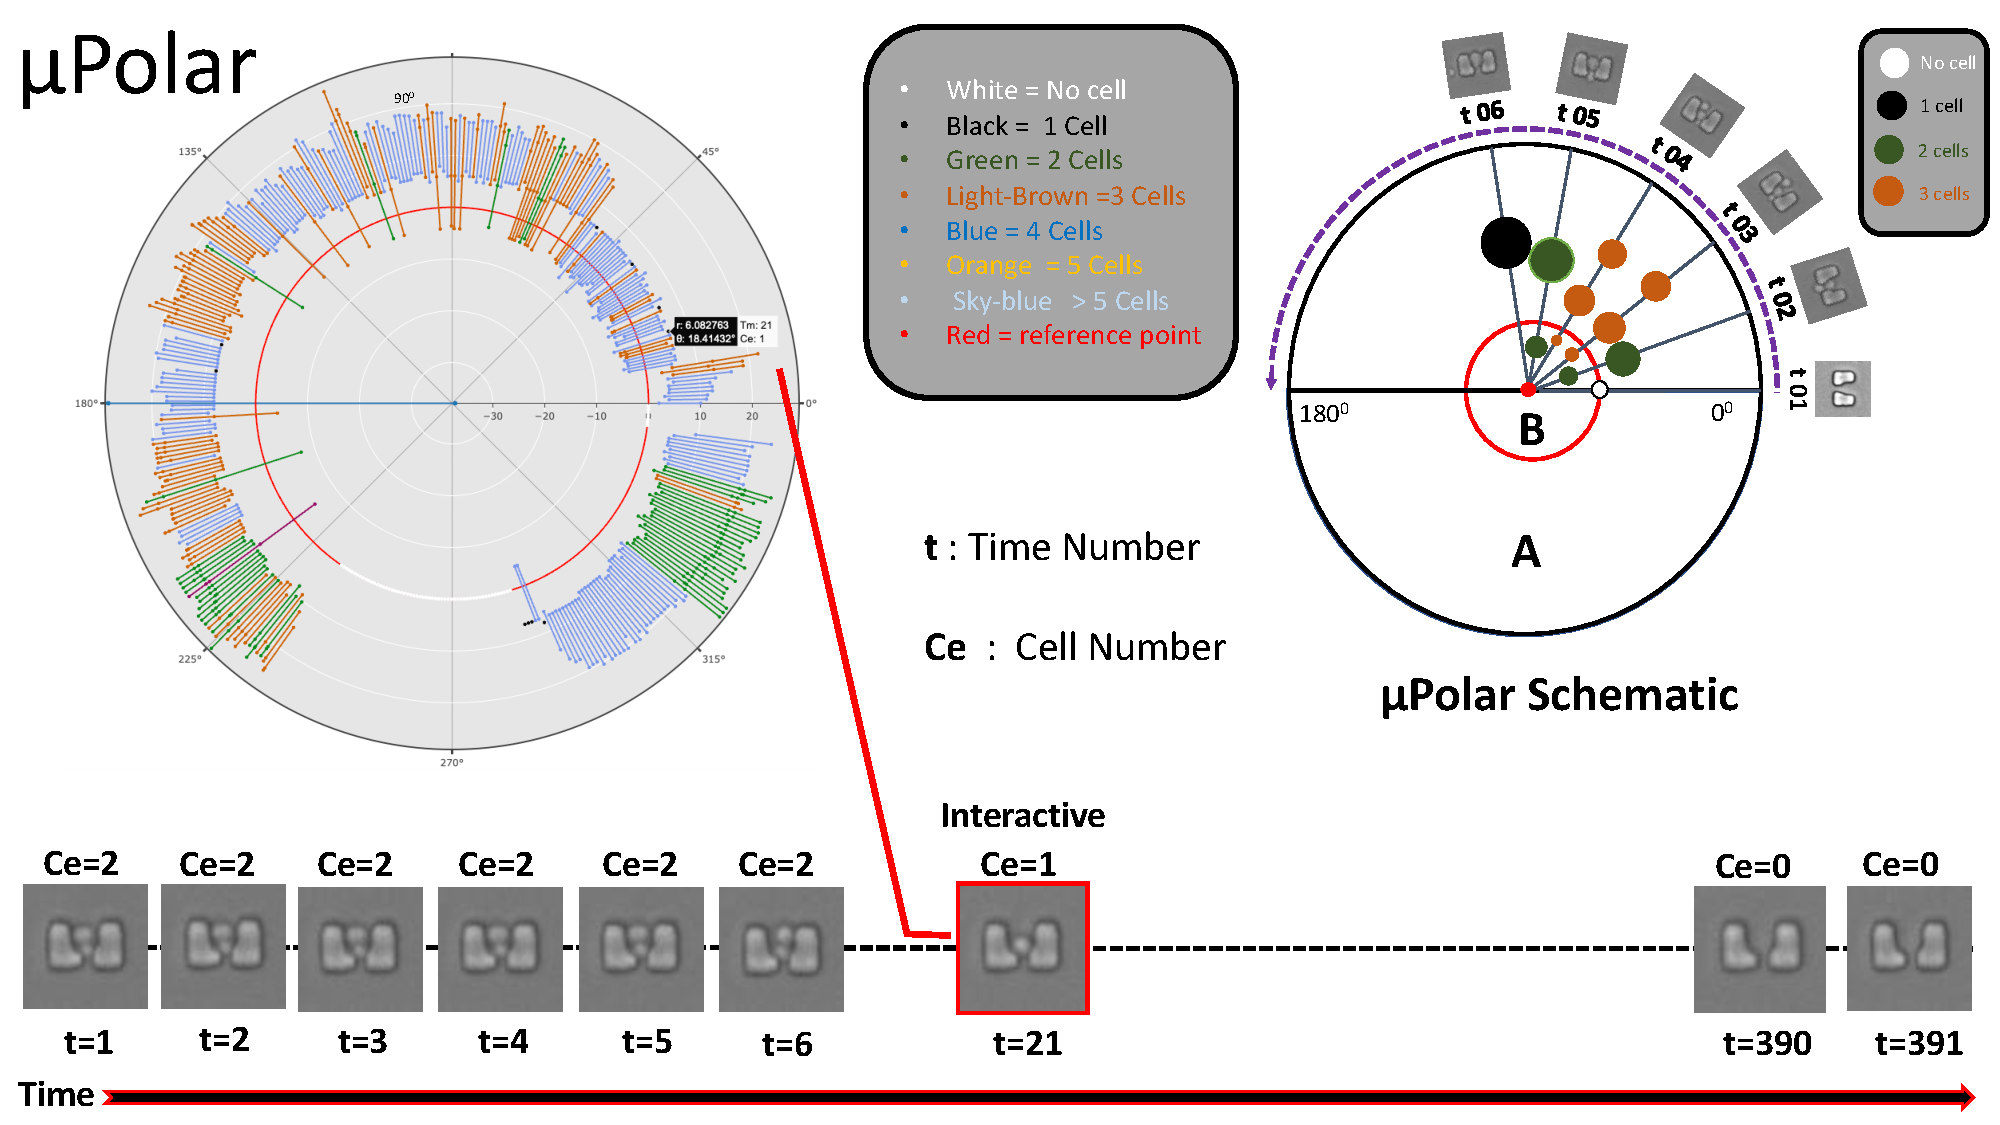
\includegraphics[width=\textwidth,height=10 cm]{Patterns/polar.pdf}
\caption{ \textbf{The design of $\mu$Polar. }. 
%A sequence of microfluidic images and dataset features including a $\mu$Polar schematic plot
(a) A sequence of microfluidic sub-images (60x60 pixels). The front image was labeled with cell numbers, coordinates, cell boundaries, and the reference point. 
(b) A sample of $\mu$Polar dataset format with optional features of area and RLS, which correspond to the front image in a. (c) $\mu$Polar plot with a representation of cell location on the plot and cell color tag. Black arrows track the same cell objects at subsequent time-points.
%%% In the image, "0 cell" should be "0 cells." Also consider capitalizing the "t" in the trap numbers, since when you spell them out elsewhere you capitalize "Trap." --BSK
}
\label{fig:table}
\end{figure*}

\subsubsection{Distance calculation}
Since the cell time-points and coordinates are available from the dataset (e.g., Fig.\ref{fig:table}b), the cell distance from the reference point  can be calculated by using the Euclidean equation

\begin{equation}
\begin{split}
d_i = \sqrt{(x_i - x_r)^2 + (y_i - y_r)^2}\\
\\
i =  [1,2,3,4,..., m ] \\
\\
\end{split}
\end{equation}

\noindent where $ d_i $ is the calculated distance at the time-point $ i $ corresponding to the image number as shown in Fig.\ref{fig:table}a and Fig.\ref{fig:table}c in light green color. $ x_i $ and $ y_i $ are cell coordinates at each image. Coordinate ($ x_r $, $ y_r $) is the reference point, which need to be specified by the user as required for the $\mu$Polar function. $ m $ is the maximum time-point equivalent to the total number of images.  The reference point could be chosen at any point of the image based on the region of interest. For instance, in Fig.\ref{fig:table}a, the reference point was chosen at $x_r = 30$ and $y_r = 1$ based on cell movement and the position of the trap.
\\

\subsubsection{Time to angular degree conversion}
The next step is to convert the image time-points to angular degrees, suitable for circular plot visualization. The time to degree conversion is calculated by

\begin{equation}
%\begin{split}
%\\
\theta = \frac{D_{max}} {T_{max}}
%\\
%\end{split}
\end{equation}

\begin{equation}
%\begin{split}
%\\
A_{acc} = \sum_{i=1}^{n}{\theta_i}
%\\
%\end{split}
\end{equation}

\noindent where $ D_{max} $ is the maximum degree (360$^{\circ}$) and  $ T_{max} $ is the maximum time-point (e.g., last time-point). $ A_{acc} $ is the accumulative angles of each radius vector ($\theta$) and $ n $ is the maximum plot degree. All cell distance values at each time-point are mapped on the radius of a circular plot with a corresponding $A_{acc}$ value.

The $\mu$Polar schematic plot in Fig.\ref{fig:table}c illustrates microfluidic images at time-point 1 (zero cells), time-point 10 (one cell), time-point 20 (two cells), time-point 30 (three cells), and time-point 40 (two cells). The color tag method represents the number of the cell corresponding to the number of cells in the image. We found this color-tagging useful to track mother cells and daughter cells at different time-points, and identify cell division events.

%cell movement interpretation. 
%%%%%%%%%%%%%%%%  how to pick reference point    $$$$$$$$$$$$$$$$$$
%We decided to choose the reference point based on cell flow direction and potential cell division point.
%Here, $ x_r $ and $ y_r $ are set to be 30 and 34 respectively at trap outlet as shown in $\nameref{Fig_S1}$. 


 %time-lapse microfluidics-based microscopic to a circular plot based on the image time and the cell distance in 2D. 
 
 % this is NOT accurate. uPloar does not detect cell objects from images
 
 % remove quotes, use italics
 
 
%Polar package, written in R language, utilizes three other R libraries, tidyverse, utils and plotly. The input of Polar are cell objects identifications, coordinates, movement measures, and timestamps. The Polar function takes time-lapse ”dataset” which only requires image ”time” and cell ”coordinate”. The dataset should be in comma-separated values (csv) format with at least ”time” and ”coordinate” features. ”Area” and ”RLS” data also could be used as additional features for the Polar visualization. Fig.1a shows a sub-image of microfluidic image (60x60) with four yeast cells inside the trap. Each cell is represented with a number and an area (circled in black). The ”red dot” represents the reference point to calculate Euclidean distance. The reference point can be chosen by the user based on investigation and limited by image dimension. Fig.1b represents the features of the dataset containing image ”time” and cell ”coordinate”. The ”area” and ”RLS ” attributes can be optionally visualized for cell monitoring and RLS analysis. In addition, Polar offers a color-based cell tracking option for cell tracking visualization.
 

%%%%%%%%%%%%%%%%%%%%%%%%%%% available color %%%%%%%%%%%%%%%%%%%
%%The $\mu$Polar" color codes are set up for 12 colors  by default categorizing the number of available cells at each time-point corresponding to cells distance. Any number above 12 would be presented as a random color. The color codes are adjustable and could be varied for different image types.  
 
 
\subsection{The $\mu$Polar R function}
The $\mu$Polar package, written in R language, utilizes three other R libraries including \textit{tidyverse}, \textit{utils}, and \textit{plotly}. The $\mu$Polar function has 10 arguments: the first argument is the input dataset, and the remaining arguments are required for visualization adjustment. Table \ref{table:desc} demonstrates an overview of $\mu$Polar function arguments. Argument (I) is the time-lapse dataset and should include \textit{Time} and \textit{coordinates}, which are required for basic visualization. The \textit{Area} and \textit{RLS} are optional features of the $\mu$Plot function and can be added to the visualization function if they are available from the dataset. Argument (II) is the reference point ($x_r$,$y_r$) that can be chosen by the user. The reference point mainly depends on the type of image and the purpose of the investigation (e.g., edge coordinate of the image in the direction of the cells'
%%% Are you referring here to the movement of one cell or multiple? If one, use cell's. If multiple, use cells'. --BSK
movement). Argument (III) is to select a particular range of time-points for plot visualization. The starting and ending time-points can be given by the user; otherwise, $\mu$Polar visualizes all time-points. This option is useful to analyze a specific range of time-points (e.g., overcrowded cells). Argument (IV) displays the plot title; otherwise, the default is no title. Argument (V) is to evenly divide the angle line on the plot. This functionality is similarly useful to analyze a range of time-points when there is an overcrowded region on the plot. Argument (VI) is a numeric value that indicates the reference line on the plot. Argument (VII) is a numerical value that adjusts the cell area when available. It represents the cell with actual size (pixels), which is useful to visualize cell movement. Argument (VIII) is vector dot colors associated with the individual cell, and the default is set to 12 colors. This option is effective to visualize cell tracking identification at each time-point. In addition, it is very beneficial for RLS analysis when the cell development can be visualized based on cell size over time. Argument (IX) is vector line colors associated with a number of cells at each time-point. This gives a good overview of a number of cells variations over time. Argument (X) adjusts the cell distance from the edge of the plot when there is overcrowding. 

%\begin{figure*}
%%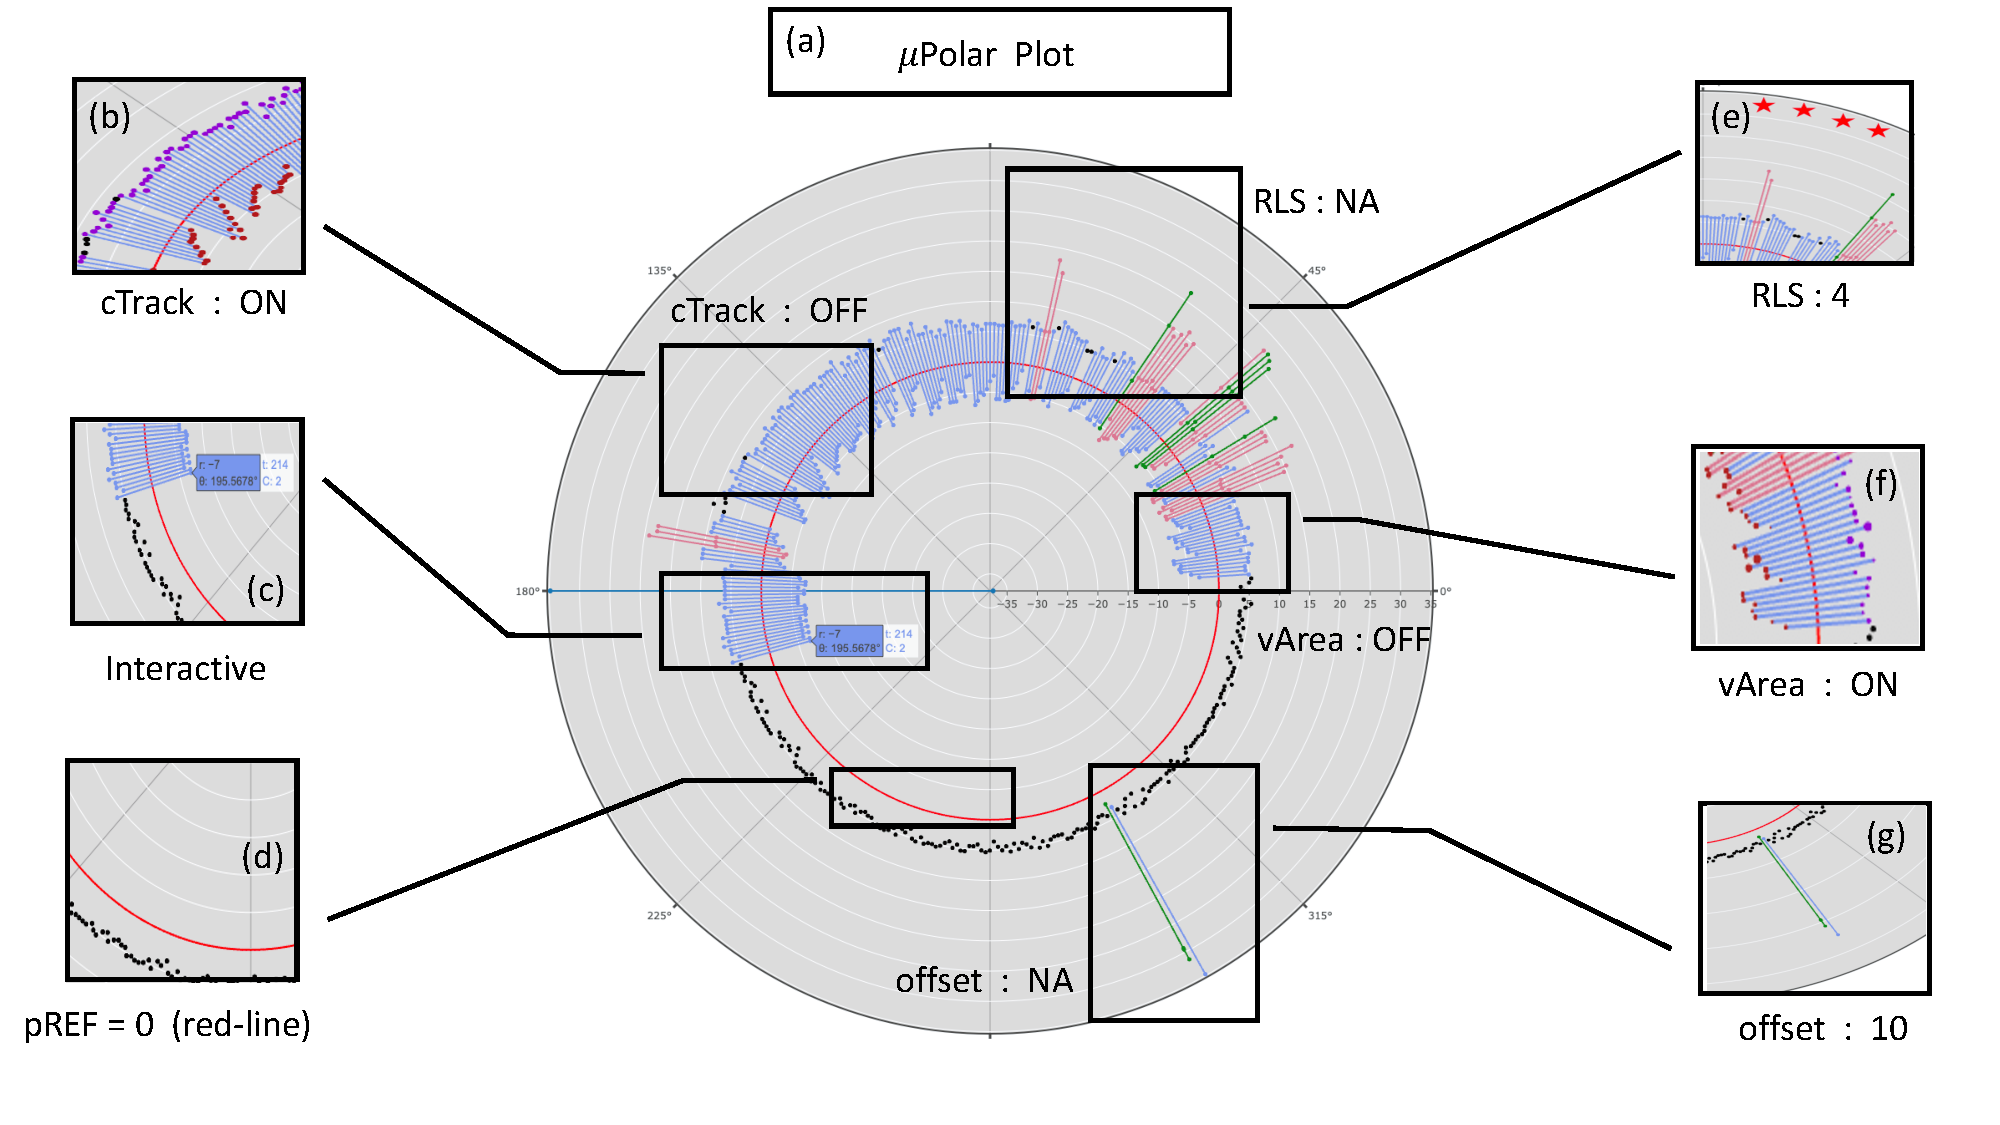
\includegraphics[width=\textwidth,height=10 cm]{Patterns/function_argu.pdf}
%\caption{ \textbf{ $\mu$Polar function inputs, time, distance, area, offset, adjust, track, and RLS}. (a) It is the $\mu$Polar plot title. (b) It shows $\mu$Polar color tracking activation when is OFF or ON. (c) It represents an interactive option in $\mu$Polar plot. (d) It illustrates the given plot reference line on the $\mu$Polar plot. (e) The RLS is available from the dataset and represented by "red star" (RLS = 4). (f) The comparison of vector area of cells when they are available from the dataset. (g) The adjustable option when cell distance is close to the edge of the plot %(offset = 10).}
%\label{fig:label}
%\end{figure*}


\begin{table*}[ht]
\caption{The $\mu$Polar R function description}
\centering
\begin{tabular}{p{0.3\linewidth}p{0.1\linewidth}p{0.5\linewidth}}
\\ 
\textbf{Function}\\
\\
\hline
\hline
\\
$\mu$Polar(sFileName,nBaseXY,nSecBE,sTitle,numAtics,nRefVal,nDotAdjust,vDotColors,vLineColors,nEdgeAdjust)\\
\\
\hline
\hline
\\
\textbf{Number} & \textbf{Argument}  &\textbf{Description}\\
\\
\hline
\\
(I) & sFilename &   Input dataset containing Time, X, Y, Area (optional), and RLS (optional)\\
\\
(II) & nBaseXY &    Given reference point ($x_r$, $y_r$) \\
\\
(III)& nSecBEt &   Given plot began and end  time-points\\
\\
(IV) & sTitle &     Plot title (default = no title)\\
\\
(V)& nNumAtics &    Number of evenly spaced angle tic lines\\
\\
(VI)& nRefVal &    Numerical value for reference line\\
\\
(VII)& nDotAdjust  &  Factor for multiplying dot size \\
\\
(VIII)& vDotColors &  Vector of dot colors associated with cell \\
\\
(IX)& vLineColors & Vector of line colors associated with linked cells  \\
\\
(X)& nEdgeAdjust &  Numerical value to extend outer plot radius\\
\\
\end{tabular}
\label{table:desc}
\end{table*}


\subsection{Representation of cell events and characteristics}
%To have a better understanding of the $\mu$Polar visualization,
We provide 8 examples to illustrate how $\mu$Polar  represent typical types of cell events and characteristics of dividing cells in microfluidics time-lapse experiments (Fig.\ref{fig:read}): traps without cells, traps with a yeast mother cells and a budding daughter cell, a cell division event in a time series,  growing mother cells with daughter cells downward, growing mother cells with daughter cell upward,  senescent and dead cells in a time series, and traps with multiple cells. 
%Several key points need to be considered for $\mu$Polar plot analysis. 
%Fig.\ref{fig:read} is an overview of some prevalent events from time-lapse microfluidic yeast cell images generated by $\mu$Polar. For example,  
Fig.\ref{fig:read}a uses a white dot on the reference line (red line) to represent a trap without cells. The red reference line is defined here at the bottom of the trap.
%%% I don't see white dots on 2a. Am I missing something? --BSK
%The black arrow represents that there is no cell at this time-point and corresponding image.
%%% This is really unclear to me. --BSK
%It commonly occurs due to shortening the cell life-cycle. The red line represents the reference point located at the trap outlet. 
The event in Fig.\ref{fig:read}b portrays
%%% Did you mean "portrays"? --BSK
the initial stage after division occurs, where the mother cell is located inside the trap with a bud at the trap outlet.  Purple dots represent the mother cell inside the trap, and the dark red dots represent the bud. The mother and daughter cells in the images are connected to their corresponding dots in the plot by arrows. In the next event Fig.\ref{fig:read}c, we highlighted a mother cell without daughter bud in the middle of a time series of mother cells with buds, indicating the moment that one daughter cell has just been separated from the mother cell, and another daughter cell is too small to be detected. 
%the black dots (black arrow) represent mother cell after its separation cycle when daughter cell increased in size and separated completely from mother cell.
Fig.\ref{fig:read}d describes a trap with 5 cells (purple line pointed by a black arrow), and an overcrowding situation that frequently occurs with growing yeast cells.
In Fig.\ref{fig:read}e, a mother cell is dividing with daughter cells budding toward the bottom of the trap. The mother cells at each time point with budding daughters are in purple, and mother cells without daughters are in black. Daughter cells budding toward the bottom of the trap are in red. 
%(purple color) remains in a steady position and daughter cell (dark red color) is at the developing stage, gradually growing in size until completing its division cycle.
Fig.\ref{fig:read}f illustrates similar cell division events except that daughter cells were budded toward the upper opening of the trap. In this case, daughter cells are in purple and mother cells are in red. 
%in the opposite cell flow direction (above reference point) when a other cell (dark red color) is located inside the trap in a steady position and daughter cell is growing gradually above mother cell. 
Fig.\ref{fig:read}g demonstrates a situation where the mother cell and daughter cell remain attached for a long period of time without detectable cell divisions. 
%have been close to each other for some time without much development. This event is considered the senescence time-point of the cell. 
Fig.\ref{fig:read}h represents a senescent mother cell that has stopped dividing. In this case, there is a single mother cell, represented in a dark dot, at each time point. 
%mother cell inside the trap, after being in a steady position for some time. 
This situation typically happens at the end of the cell lifespan.
\begin{figure*}
\centering
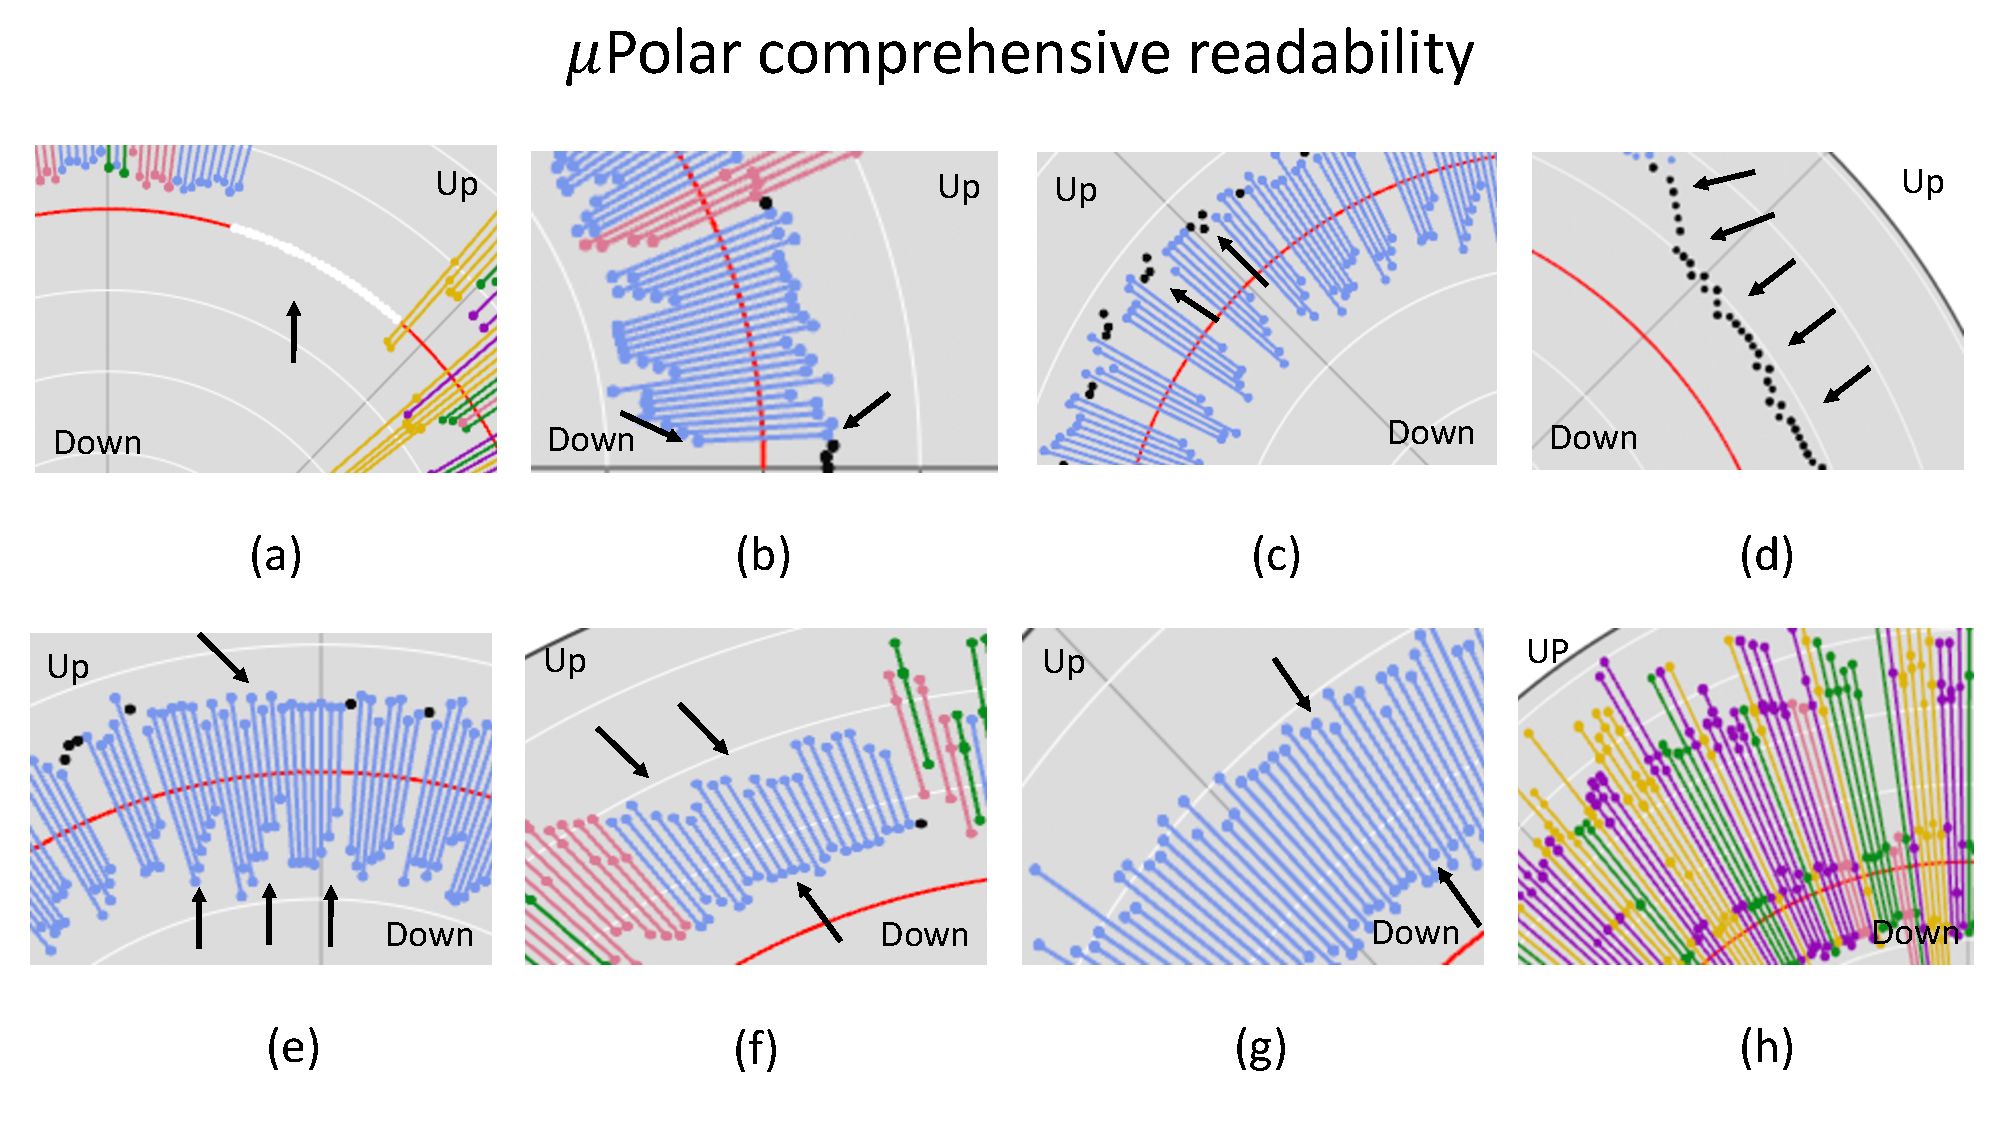
\includegraphics[width=\textwidth,height=10 cm]{Patterns/read.pdf}
\caption{\textbf{ Typical cell events visualized by $\mu$Polar}. Any events that occurred below the reference line (red) are denoted as ``down,'' and any events that occurred above the reference line (red) are denoted as ``up.'' (a) There is no cell at the presented time-point (white dot).
%%% Again, I don't see white dots. --BSK
(b) The two cells represented by dark red dots and purple dots are close to each other, and division already happened. (c) The black dots represent a division after the cell completed its separation cycle. (d) Indication of overcrowded cell events. (e) Representation of steady cells in the up region (purple color) and developing cells in the down region (dark red color). (f) Representation of steady cells in the up region (dark red color) and developing cells in the up region (purple color). (g) Two cells are in a steady situation for some time, an indication of senescent cells. (h) The representation of a cell that has been dead for some time. }
%%% In sub-image d, "UP" should be "up." And can you move "Down" a little down and to the right, so more of it is in the grey space? Right now it's difficult to read and easy to miss entirely. --BSK
\label{fig:read}
\end{figure*}


\section{Package availability}
The package $\mu$Polar is an open-source package freely available on Github at https://github.com/merang/uPolar. The package installation can be done in R either using the install\_github function in the ‘devtools’ or using the githubinstall function in the ‘githubinstall’ package. 

%The R code for installation of $\mu$Polar package using the ‘devtools’ package is as follows: \\
%\\
%install.package("tidyvers")\\
%\\
%install.package("R.utils")\\
%\\
%install.package("plotly")\\
%\\
%libarary(devtools) \\
%\\
%install\_github$("https://github.com/merang/uPolar")$\\
%\\

\section{Data Used}
 To demonstrate $\mu$Polar's utility, we plotted two sets of time-lapse microscopic images: one set of dividing yeast cells and the other of migrating mouse fibroblasts. The yeast  cell images were generously provided to us from a recent experimental work in  \cite{r13}.  The original microfluidic images contain many traps , we partitioned these images into 391 sub-images in 60x60 pixels dimensions based on the cell traps. The mouse fibroblast dataset is publicly available and contains 37 time-lapse microscopic images \cite{r20}. Since the number of fibroblast in each image (307x306 pixels) was more than 50, we cropped a section of time-lapse images in 121x121 pixels dimensions. Based on image size and resolution, the $\mu$Polar function can be applied to any time-lapse cellular microscopic images by cropping the region of interest. Image feature extraction (e.g., coordinates, area) can be done via many methods. We used ``Fiji - ImageJ'' tools to obtain cell coordinates and cell area. This process can be automatic; however, it often need manual verification especially for  images with low resolutions. The obtained data can be exported in CSV format, which is suitable as inputs for $\mu$Polar.  

%%%%%%%%%%%%%%%%%%%%%%%%%%%%%%%%%%%%%
%       add video link for user  
%%%%%%%%%%%%%%%%%%%%%%%%%%%%%%%%%%%%

\section{Results}
%We have applied the $\mu$Polar visualization package to two sets of images; time-lapse microfluidic images of yeast cells and time-lapse microscopic images of mouse fibroblasts. The microfluidics sequence images are procured from \cite{ref13} recent experimental work. Since microfluidic images had low resolution (1280x960), we partitioned the image to time-lapse (1-391) sub-image of 60x60 dimension. Furthermore, we collected 37 time-lapse microscopic images from \cite{ref05} as a different type of dataset to test on. For visualizing the microscopic images, we cropped a section of time-lapse images from 307x306 to 121x121 dimensions. Base on image size and resolution, $\mu$Polar function can be applied to any time-lapse cellular microscopic images by cropping the region of interest.    

% add video link for data collection  %%%%%%%%%%%%%%%%%

\subsection{Application to  microfluidic yeast cell images}
We present 10 $\mu$Polar plots for Trap No. 2, 12, 22, 41, 50, 59, 73, 82, 98 and 100 in \nameref{Fig_S1}. These 10 plots represent a range of cell division events. 
%Several microfluidic image traps are shown in \nameref{Fig_S1}, including Trap 2, Trap 12, Trap 22, Trap 41, Trap 50, Trap 59, Trap 73, Trap 82, Trap 98, and Trap 100. 
%We chose these traps based on the investigation of cell development at the beginning, middle, and end of the microfluidics device. 
In each image, we use color to represent the number of cells in each trap. 
%Each color represents several cells in a range of 1 to 6 in an individual image. 
The white, black, light blue, pink, green, purple, and orange colors represent 0 cells, 1 cell, 2 cells, 3 cells, 4 cells, 5 cells, and 6 cells, respectively.

Additionally, we provided three zoomed-in examples.  
%evaluated some $\mu$Polar plots from different trap numbers at different time-points with the corresponding image. For instance, \nameref{Fig_S2}
%%% Having these show up as "S2 Fig" vs. "Fig S2" feels wrong. If you decide to switch to the latter, be sure to catch all instances. --BSK
In \nameref{Fig_S2}, we highlighted time-point 30 of Trap No. 8, which contains 4 cells above the tap, represented in a green line. 
% Figure S2 is a bad example of 3-cell objects. 
%shows $\mu$Polar visualization of Trap8 at time-point 109. The plot indicates three cells (pink color) in the image: 
At this time-point, all cells are above the reference line and a cell division happened outside the trap due to the oversized mother cell (\#4). In another example, \nameref{Fig_S3} demonstrates Trap No. 33 at time-point 11 when there are 2 cells available in the image. This is an early stage of cell division when 2 cells (sky blue line) are very close to each other. In \nameref{Fig_S4}, we show the oscillating plotting patterns that represent regular cell division intervals of an healthy yeast mother cells in the initial one-third of the plot. \nameref{Fig_S4} also shows a scenario of likely senescent cell in Trap No. 63 at time-point 340, in which a single mother cell has remained undivided for almost two-third of the microfluidic experiment period.

In \nameref{Fig_S5}, we illustrate how we can change the reference point $(x_{r},y_{r})$ to visualize the time series from different perspectives, using Trap No. 44 as an example. \nameref{Fig_S5}a represents a $\mu$Polar plot when the reference point is (0, 0). This representation is only based on the cell centroid point coordinates without the distance calculation. \nameref{Fig_S5}b represents a $\mu$Polar plot when the reference point is (30, 60). This representation is based on the distance calculation. The comparison of selected regions (black box) portrays that cell variations are more visible in  \nameref{Fig_S5}b. Therefore, selecting the right reference point is an effective factor to improve the division time-points countability on the plot.

\subsection{Application for microscopic mouse fibroblast images}
 To demonstrate its general utility, we applied $\mu$Polar to a data set of time-lapse microscopic images of  migrating mouse fibroblasts (Fig.\ref{fig:scopic}a). The number of available cells in each image is in a range of 50 to 70 depending on the time-point. The average cell size is bigger than the average yeast cell size. For simplicity, we focused on a section of these images as illustrated in Fig.\ref{fig:scopic}b. Correspondingly, feature extraction is applied to these images, collecting cells coordinate of each image in order of time. According to our observations, cells gradually migrate from the right side to the left side in these images over time. Thus, we chose the reference point at the left side of the image edge ($x_r$ = 2 pixels, $y_r$ = 60 pixels) for distance calculation. In Fig.\ref{fig:scopic}c, we used a unique color to represent the same cell object at each time point. We like to emphasize that the changing diameters of colored dots represent the changing cell shapes during migration. In addition, each color represents the cell number at each time-point. For example, the orange color at time-point 37 illustrates that there are 9 cells at this time point and the orange dot is the cell number 9 at this time-point. 
 %illustrates the $\mu$Polar plot where the cell numbers are in a range of 6 to 10 in each time-point and indicated by different colors. Each colored dot represents a tagged cell with numbers 1 to 10.  

\begin{figure*}
\centering
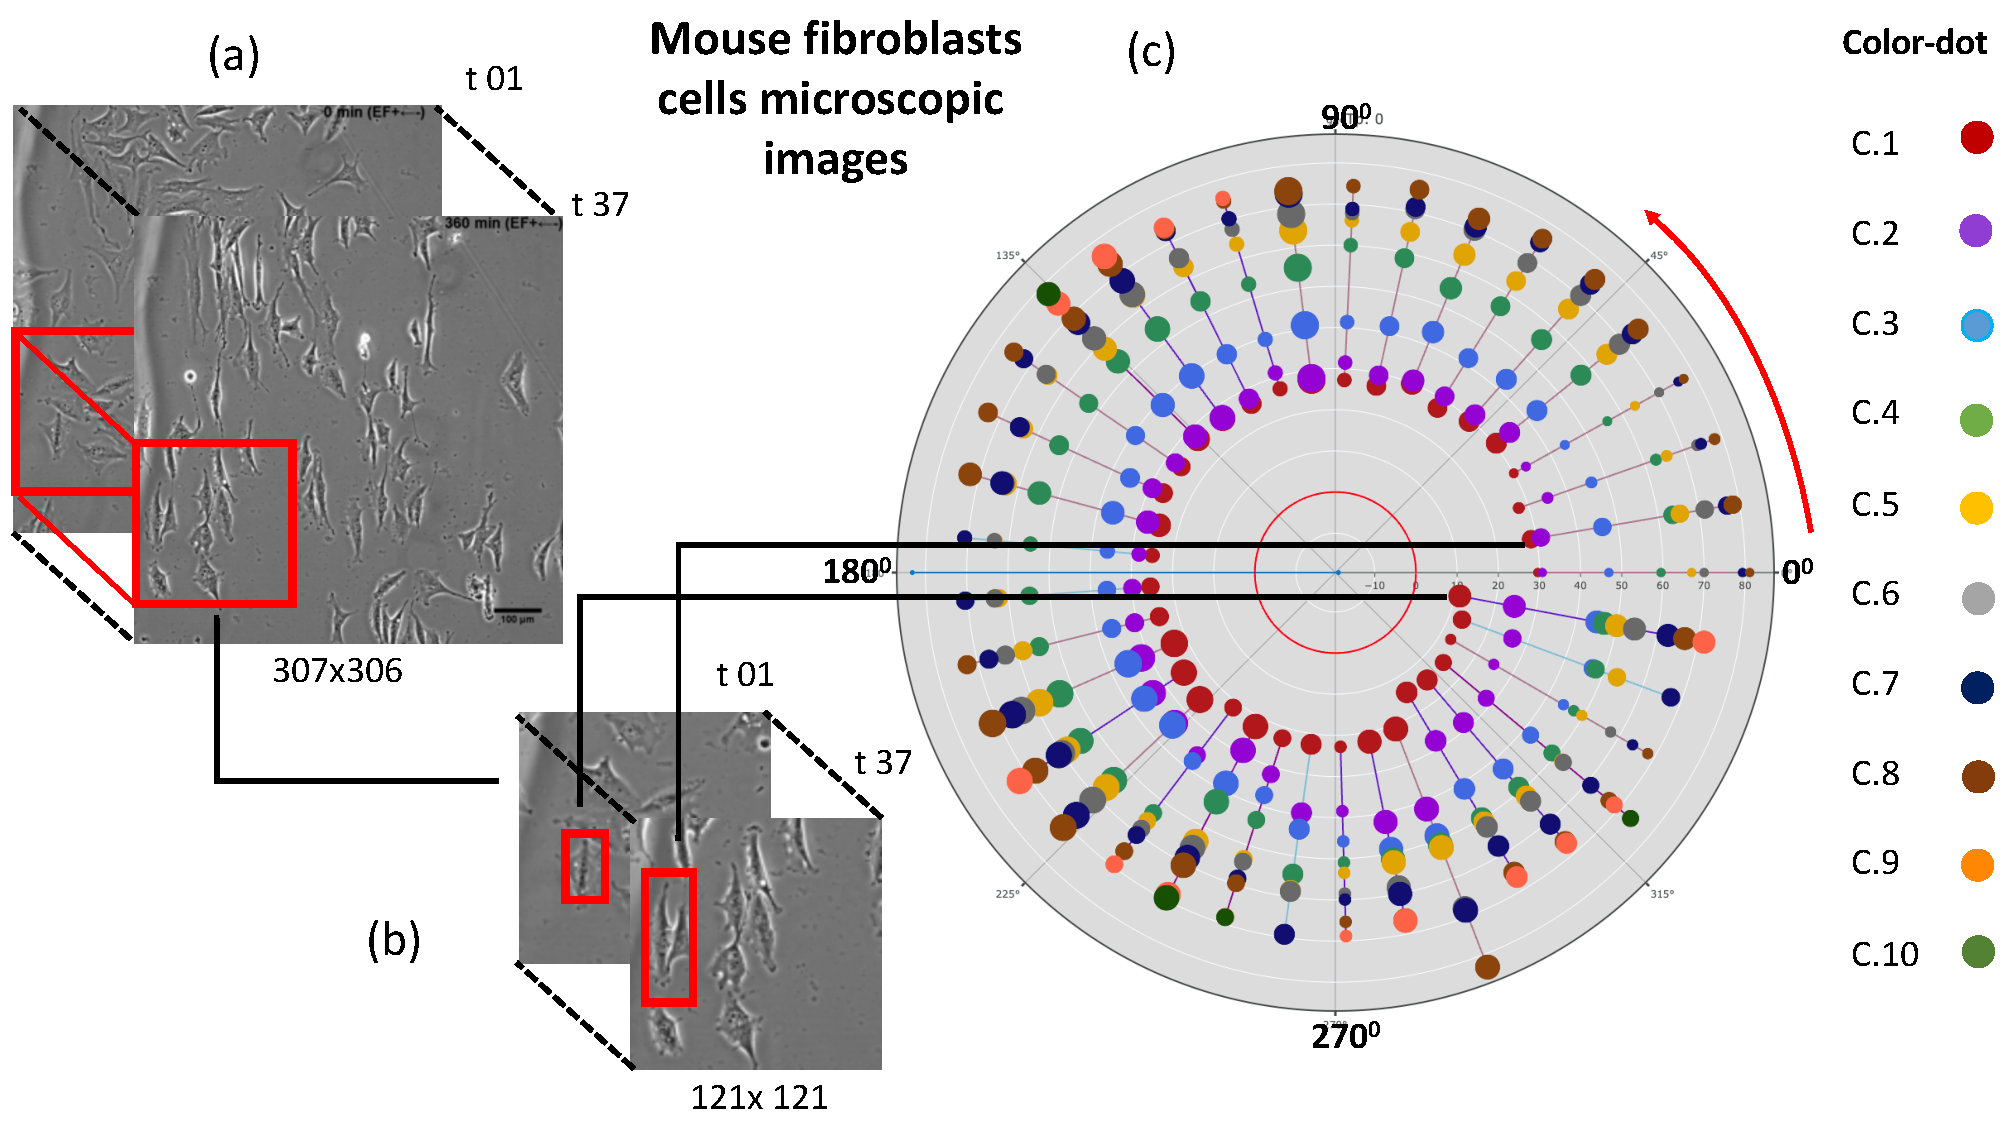
\includegraphics[width=\textwidth,height=10 cm]{Patterns/microscopic.pdf}
\caption{ \textbf{$\mu$Polar plot for migrating mouse fibroblast cells in time-lapse microscopic images}. Cell areas are represented by dots with variable diameters, and the same cell objects in each time point are marked by a unique color. 
%and color tag tracking are applied for this plot. Cells are represented with colored dots at each time-point.
%%% (1) In the title, "fibroblasts" should be singular. (2) the trap numbers should not have a space between the "t" and the number, to be consistent with similar formatting throughout. (3) In the upper right, "Dot color" should be "Dot color." --BSK
}
\label{fig:scopic}
\end{figure*}

%\subsection{ Cell size variation and color tracking }
\subsection{Representation of cellular characteristics and movement }
Cellular characteristics such as cell sizes and movements are informative to illustrate biological processes such as aging. $\mu$Polar function has an option to import cell size information (area) for visualization. 
%otherwise, all the cells are represented by default size (5 pixels). 
%The representation of cell variation is critical to identify the cell division time-points, and very useful for counting RLS. The cell size variation and cell tracking are based on the color tag method in the $\mu$Polar plot. 
In general, there are two sets of color representation in the $\mu$Polar plot: colored lines and colored dots. The colored lines represent the numbers of cells detected at each time-point and are often displayed in lighter colors. The colored dots representing individual cells at each time-point and are often displayed in darker colors.

Fig.\ref{fig:scopic}c is an example of cell size variation. The cell movement and development can be determined by following a cell with the same color at each time-point. For instance, the comparison between the closest cell to the center-point at time-point 1 (dark red dot) and the closest cell to the plot center-point at time-point 37 (dark red dot) shows that the cell migration from time-point 1 to time-point 37 is approximately 20 units. 
%Since the total number of images is 37, $\mu$Polar color tag indication shows a great visualization of cell movement and size variation. 

 
\begin{figure*}
\centering
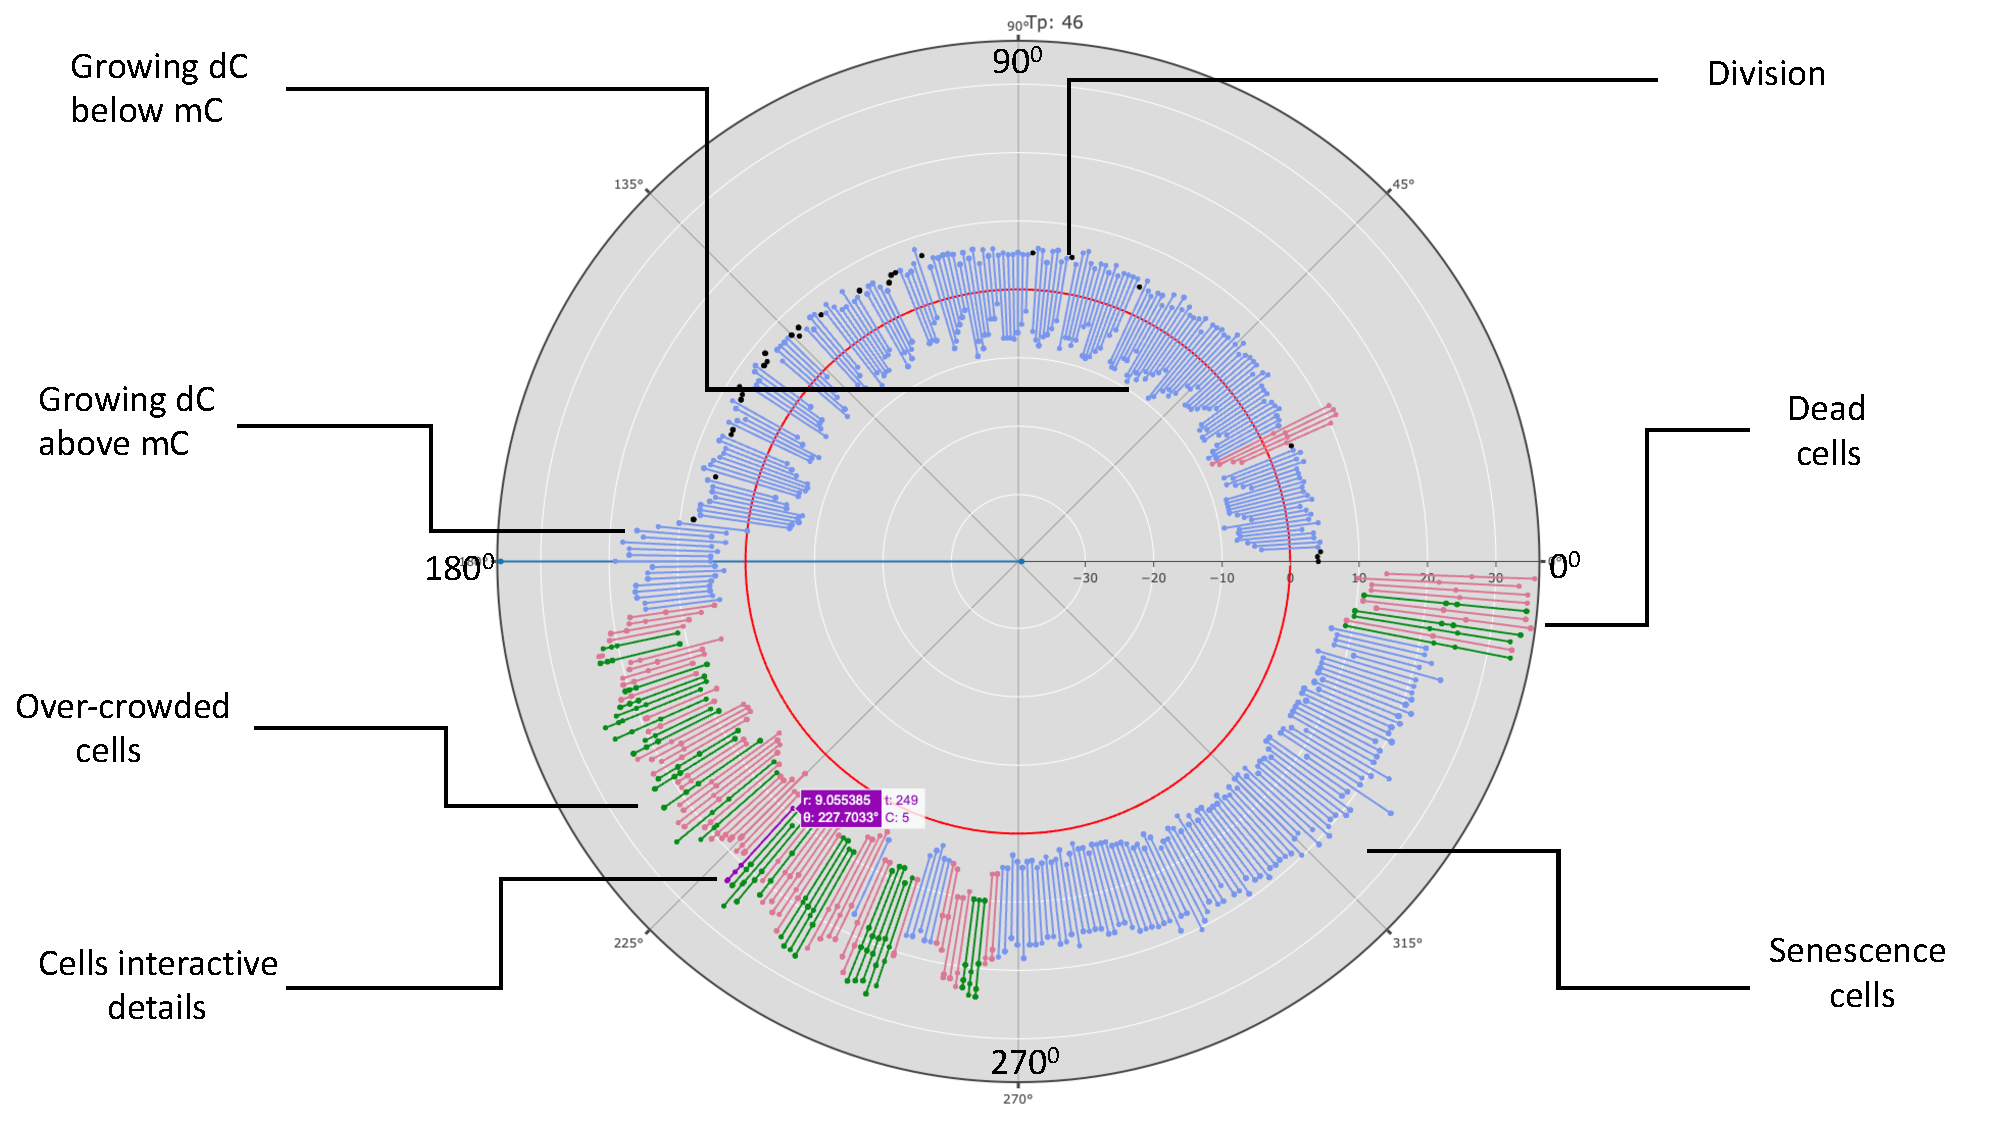
\includegraphics[width=\textwidth,height=10 cm]{Patterns/explain.pdf}
\caption{ \textbf{ A $\mu$Polar plot with cell area representation and cell tracking for Trap No. 98}. The line color represents the number of cells at each time-point, and dot color represents a color tag for individual cell at each time-point, respectively.
%%% (1) In the legend in the upper left, the line labels are misaligned, aka "cells" doesn't line up across all four. (2) The caption on #5 needs to be moved down a little. (3) There's an extra space in the caption on #2. (4) In the upper right, "Dot color" should be "Dot color." "Line color" should be "Line color." (5) "Senescence" should be "senescent." --BSK
}
\label{fig:explain}
\end{figure*}

Fig.\ref{fig:explain} is a $\mu$Polar plot with cell area and color tracking for time-lapse microfluidic images of dividing yeast cells. Here, the numbers of cells at each time-point are in a range of 1--5 cells Cells can be visually tracked based on colored dots and cell size variation, which can assist the determination of cell division events.
%Fig.\ref{fig:explain} represents the Trap No. 98 from \nameref{Fig_S1}. Fig.\ref{fig:explain} shows the number of cell objects detected at each time-point are in a range of 1-5 cells. 
%where black dots represent one cell and colored lines represent 2--5 cells at each time-point. 
%It can be seen that the number of cells is 2 for most of the time-points. 
The \text{\textit{\#1}} scenario shows that there was a single cell (black dot) in the previous time-point and there is a mother cell (purple dot) with developing bud (dark red dot) at the present time-point. 
%This is a \textbf{\textit{daughter cell below mother cell}} situation, when mother cell (purple dot) is inside the trap and daughter cell (dark red dot) is growing in the direction of microfluidic medium flow direction at trap outlet.
The \text{\textit{\#2}} scenario illustrates a single mother cell with a daughter cell growing upward. 
%that after some time, there is a \textbf{\textit{daughter cell above mother cell}} situation when a single mother cell (dark red dot) is inside the trap and a daughter cell (purple dot) is developing in the opposite direction of microfluidic medium flow direction. The order of colored dots is based on the closest cell to the plot center point. This can be changed from time-point to time-point;
%however, similar cells can be identified based on the position at their time-points. Thus, the purple dots and dark red dots at \text{\textit{\#1}} and \text{\textit{\#2}} indicate the same mother cell based on its position on the plot. Between these time-points, there are small variations in the number of cells (colored line) for a short period and followed by 2 cells again. This process continued for some time and the number of cells increased (colored line) from 2 cells to 3 cells for a longer period until there were not any cells available inside the trap as represented at event \text{\textit{\#3}}. After this transition (2 cells to 3 cells), the division started again with a \textbf{\textit{daughter cell below mother cell}} event and continued longer than a similar event at earlier time-points.
The \text{\textit{\#3}} scenario indicates an empty trap. In this case, the previous yeast mother cell has been washed away. 
Scenario \text{\textit{\#4}} represents the transition 2 cells to 1 cell, indicating a completion of a cell division. 
%These division cycle points have occurred several times in this example. The division countability is useful to estimate the number of divisions by visualization. 
Scenario \text{\textit{\#5}} shows that a daughter cell (dark red dot) is growing below a mother cell (purple dot). 
Scenario \text{\textit{\#6}} represents an overcrowded situation. 
%These cells can be tracked down by corresponding color and size variation at each time point. Cells at overcrowded time-points can also be identified by corresponding Dot colors as illustrated in \text{\textit{\#6}}.
Scenario \text{\textit{\#7}} is an example of a senescent mother cell whose cell division took a long period of time, probably because the daughter cell is extremely elongated.
%Senescence time-points in \text{\textit{\#7}} are demonstrating that 2 grown cells (dark red dot and purple dot) have been closed to each other for some time without noticeable variation in cell size or division point. 
Scenario \text{\textit{\#8}} represents a single cell inside the trap close to the end of the experimental work and is likely a dead cell. 

We would like to emphasize that other cellular characteristics, such as morphological aspect ratio, can be visualized in $\mu$Polar as well. 

\subsection{Counting RLS and interpretation of experimental results}
$\mu$Polar has an additional option to visualize the replicative lifespan. This feature can be added to the plot if RLS data is available from the dataset. The RLS division point is represented as a red star at corresponding time points.  
%%% Wording feels off here. What does this mean? --BSK
%with a red star. 
Circular plots of dividing cells can visualize the cell division events in oscillating patterns.  Fig.\ref{fig:rls} demonstrates the RLS comparison between given RLS information and counting RLS from $\mu$Polar plot division points without prior information. We previously collected the experimental RLS data for each trap from \cite{r13} and applied this information to the $\mu$Polar plot. The red stars in Fig.\ref{fig:rls} represent 21 cell divisions from experimental results. The black arrows inside the plot represent the cell division events estimated from $\mu$Polar plot analysis, counting 22 cell division events. 
The estimation based on the circular plot is nearly identical to the experimental result except at one time-point indicated by a question mark. 
The oscillating patterns of the first 17 cell divisions are visually striking, representing that daughter cells gradually grow larger in size and then separate from the mother cells at regular intervals -- a characteristic of a healthy yeast mother cell. 
Although there are some overcrowded time-points and large cells in the second half of the plot, this plot demonstrates the utility of circular plots in RLS estimation. 
%the region of interest and range of time-points for counting RLS.       

\begin{figure*}
\centering
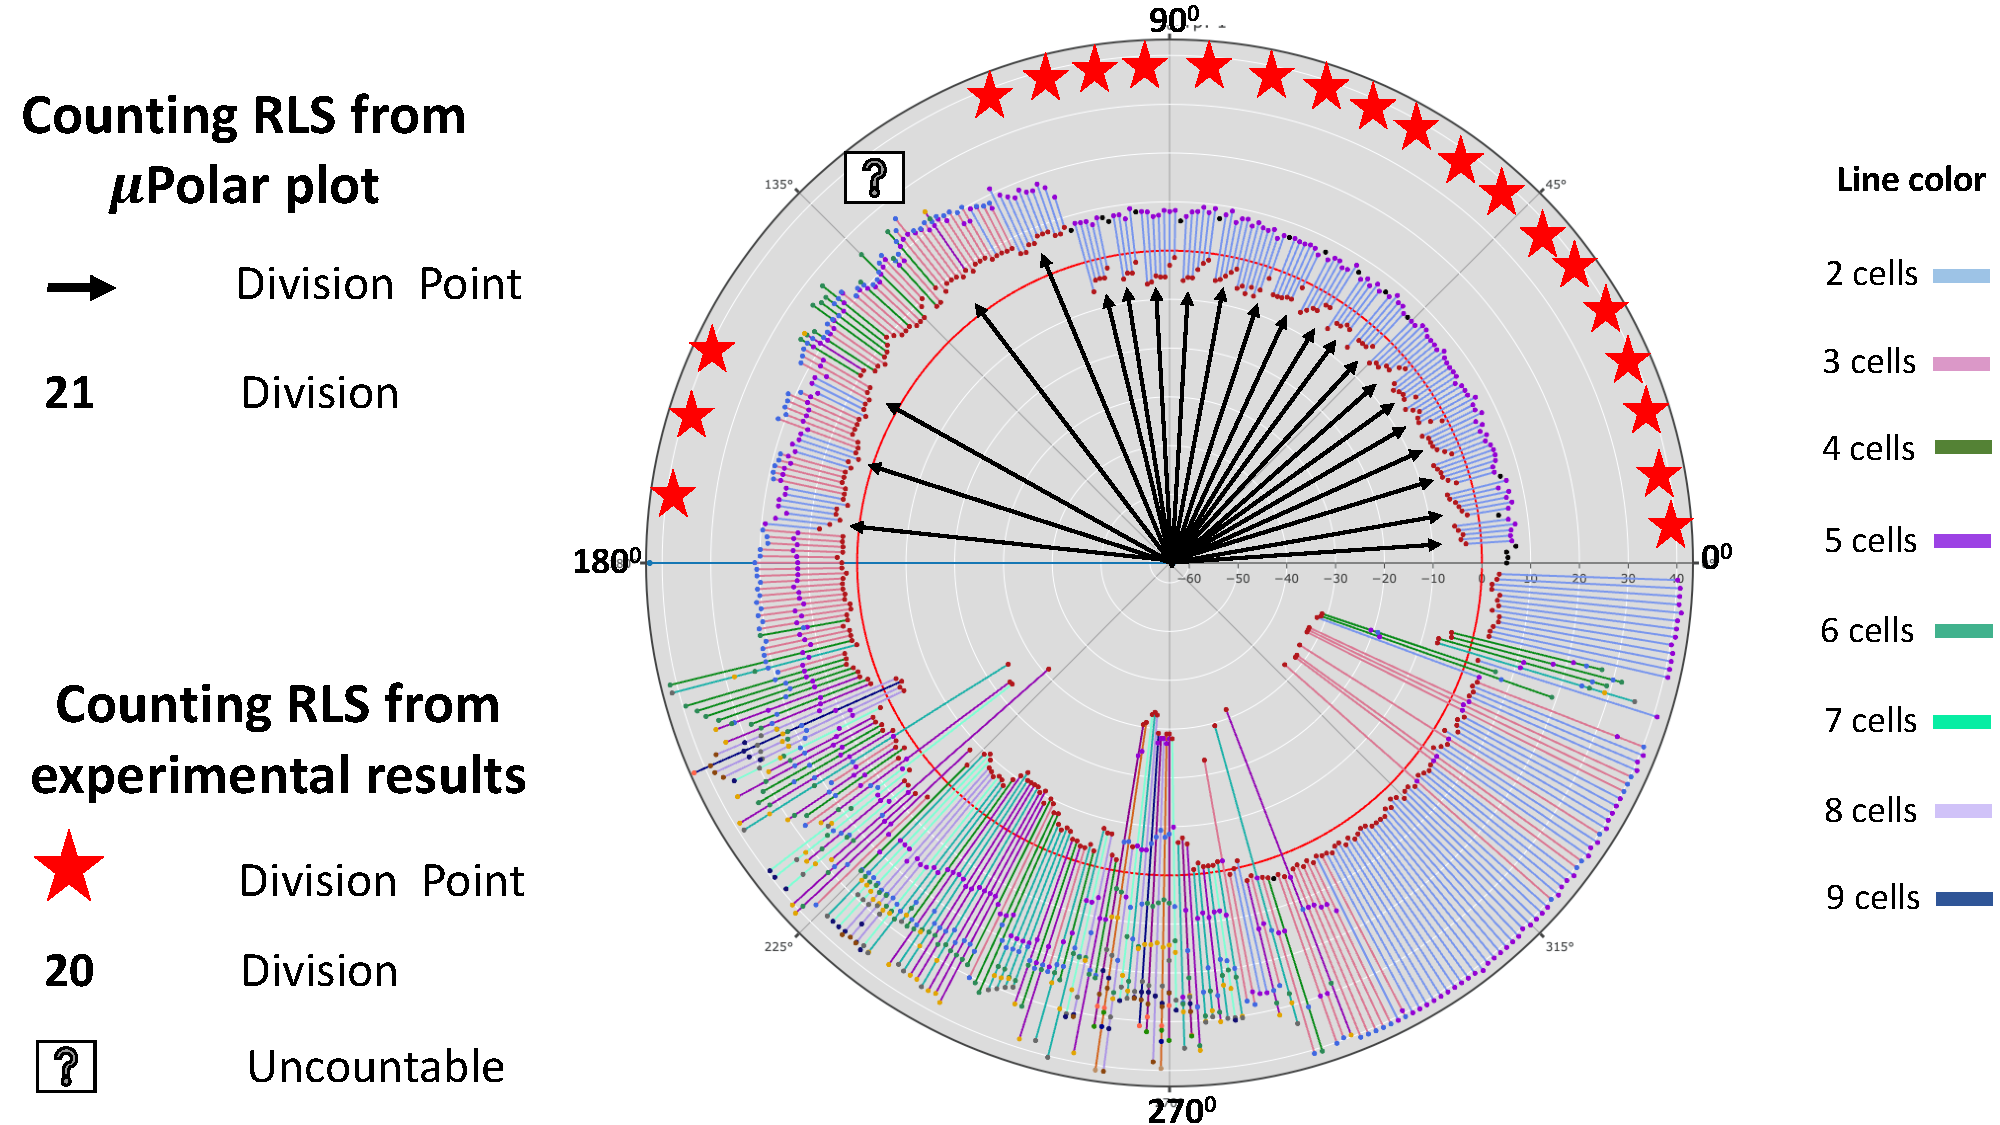
\includegraphics[width=\textwidth,height=10 cm]{Patterns/rlsTp1.pdf}
\caption{ \textbf{Identifying RLS measurements from $\mu$Polar plot for Trap No. 1}. The black arrows indicate the potential number of yeast cell division time-points from $\mu$Polar plot estimating 22 divisions. The red stars indicate the 21 cell division events identified from the experimental results.
%%% (1) There's an extra space in the first title. (2) As above, "cells" doesn't align on the line labels in the legend on the right. (3) "Line color" should be "Line color." --BSK
}
\label{fig:rls}
\end{figure*}

%In this section, the simplicity and practicality of the $\mu$Polar tool in the contour expansion will be discussed
\section{Discussion}

Overall, $\mu$Polar is a useful tool for visualizing cell migration, cell monitoring, and estimating cell division events from time-lapse microscopic images. The $\mu$Polar interpretation of cell division at each time-point can facilitate lifespan estimation in aging studies. The comparison between yeast cell time-lapse microfluidics images and mouse fibroblast cell time-lapse microscopic images demonstrates that $\mu$Polar can be a general tool for visualizing time-lapse images.

Visualizing cell division events can offer biological insights. 
For instance, in the microfluidic images, it can be seen that when yeast cells become older, interestingly, the cell division cycle becomes longer. It can also be seen that there is a relationship between cell size and cell division time-length. Similarly, visualizing and tracking mouse fibroblast cells show how cell sizes change during their migration. 
%Potentially, $\mu$Polar could be a great visualization tool to compare a cell separation cycle time at its early lifespan and cell separation cycle time at its late lifespan. 
%Moreover, $\mu$Polar can be a useful tool for microfluidic device design prospective in terms of quality evaluation, trap location, and shape. 


%\section{future work}

 %package limitation 
 
% Despite these contributions, our models also has multiple limitations
% that provide useful opportunities for future work.
% First, a major limitation of binning observations into the four
% time bins is loss of information on short-term irregularities. For instance,
% conditions such as heart arrhythmias can only be identified
% when analyzing high resolution heart rate data. Averaging all values
% within 8h bins removes any such high resolution patterns. Furthermore,
% the DeepObserver model is difficult to interpret by medicine
% practitioners being black-boxed in nature. Future research should
% aim at producing more interpretable version of DeepObserver.
% Second, ClinicalBERT_Multi use clinical notes to predict CCS
% categories, thus inheriting all limitations from the ClinicalBERT

%\section{Conclusion}
Time-lapse microscopy is becoming an increasingly popular research tool to monitor cellular events in biomedical research. One such application is the microfluidics-based high-throughput analysis of dividing yeast cells. It is challenging to visualize and interpret the large volumes of data gathered through microfluidics-based microscopy. Here, we developed a circular plotting method, $\mu$Polar, to visualize cell movements and cellular division events at hundreds of time points. Our method is interactive and easy to use. We demonstrated the utility of our method to describe the events of dividing yeast cells and migrating mouse fibroblast cells. Our method could be applied to other types of microfluidic devices and time-lapse microscopic imaging experiments.

%This software is implemented in an R package $\mu$Polar available through GitHub from https://github.com/merang/uPolar.
\
\section{Supplemental Information}

\paragraph*{Fig. S1}
\label{Fig_S1}
{
%%% All of these supplemental figures have different captions for the same thing. Pick one wording and make them match. --BSK
Time-lapse full microfluidic images with $\mu$Polar plots for Trap No. 2, 12, 22, 41, 50, 59, 73, 82, 98 and 100}. 


\paragraph*{Fig. S2}
\label{Fig_S2}
{Visualization of Trap No. 8
with a corresponding microfluidic image}. 

% \begin{figure*}
% \centering
% 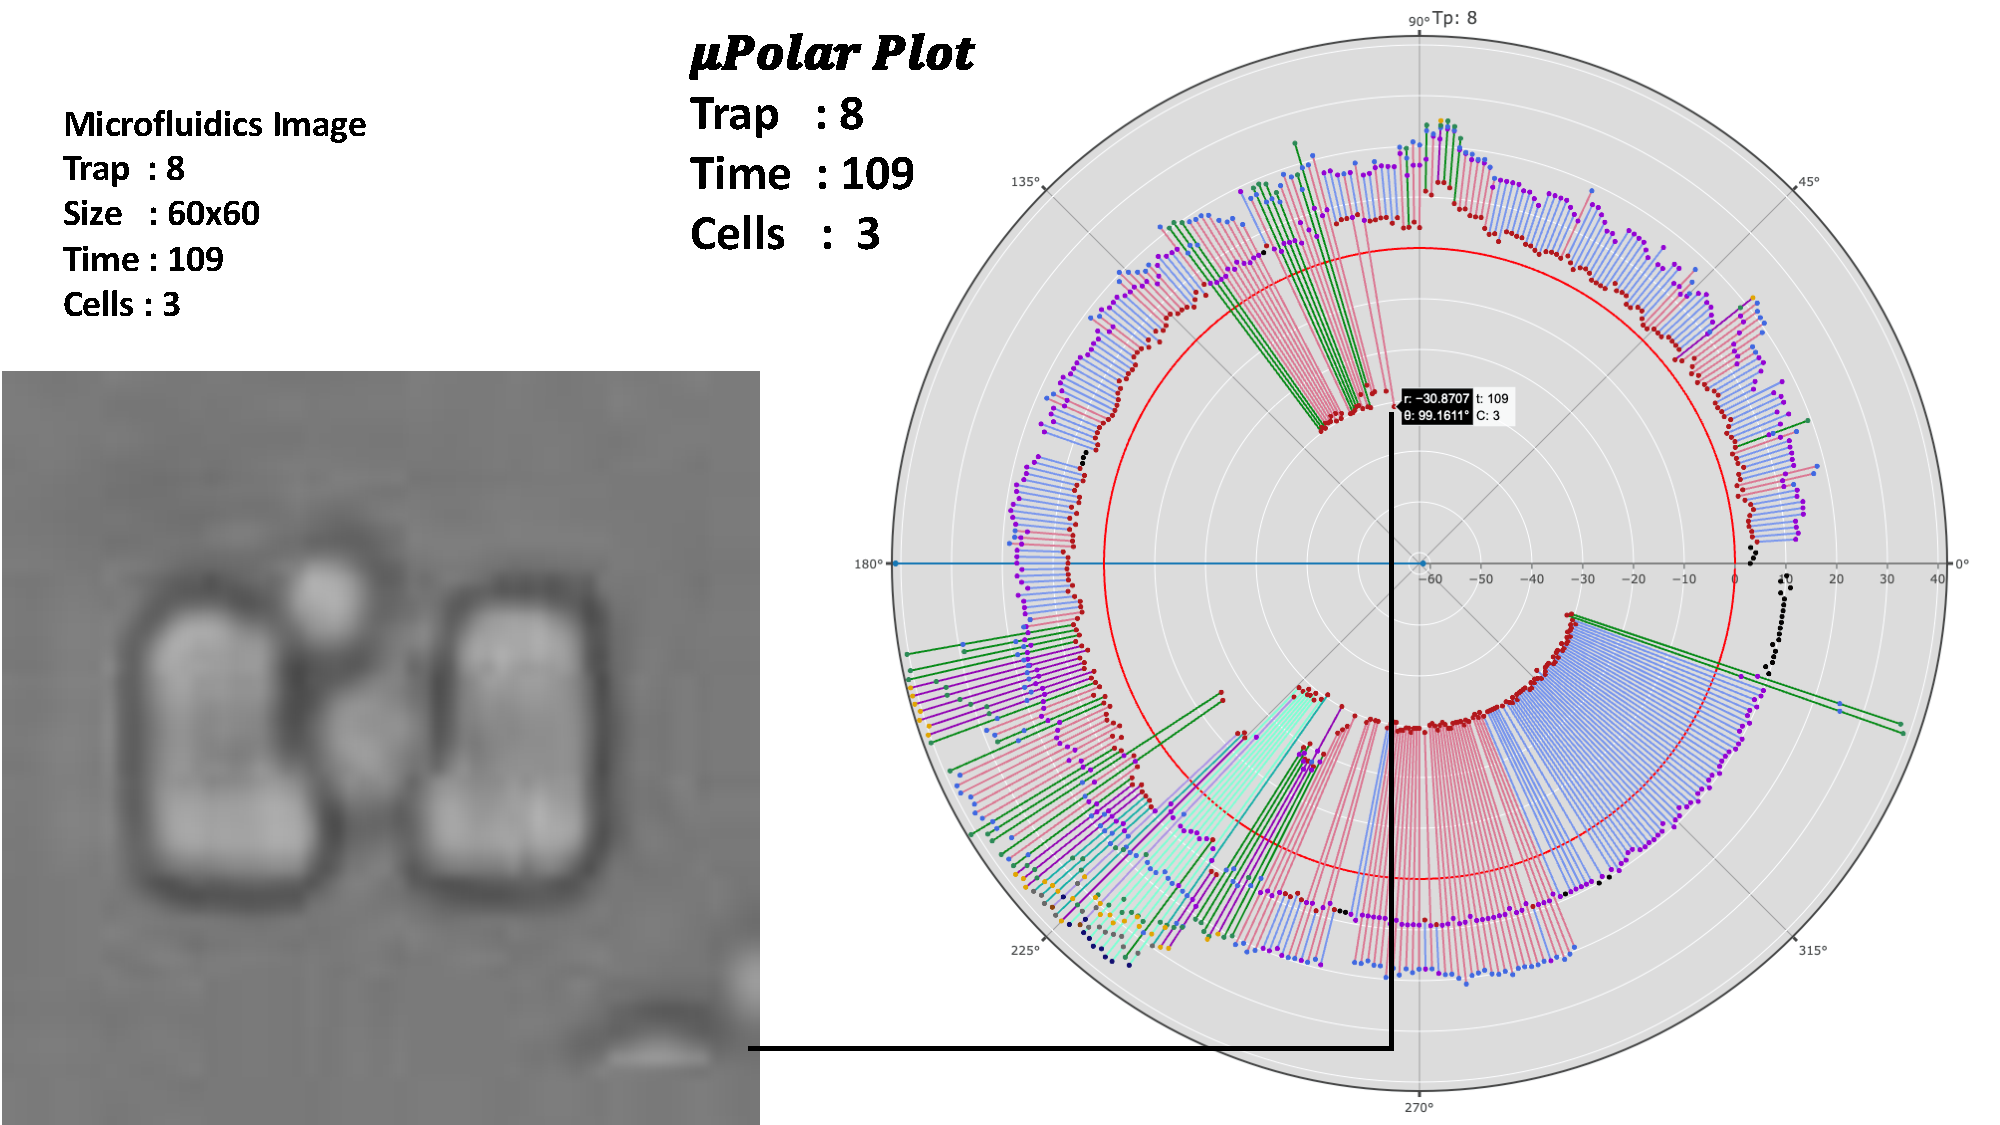
\includegraphics[width=\textwidth,height=10 cm]{Patterns/bc8tp8.pdf}
% \caption{ \textbf{$\mu$Polar visualization for Trap08 microfluidics images}.}
% \label{Fig_S1}
% \end{figure*}

\paragraph*{Fig. S3}
\label{Fig_S3}
{ Visualization of Trap No. 33 with a corresponding microfluidic image.
%%% Missing colon in the trap number under the title. --BSK
}

% \begin{figure*}
% \centering
% 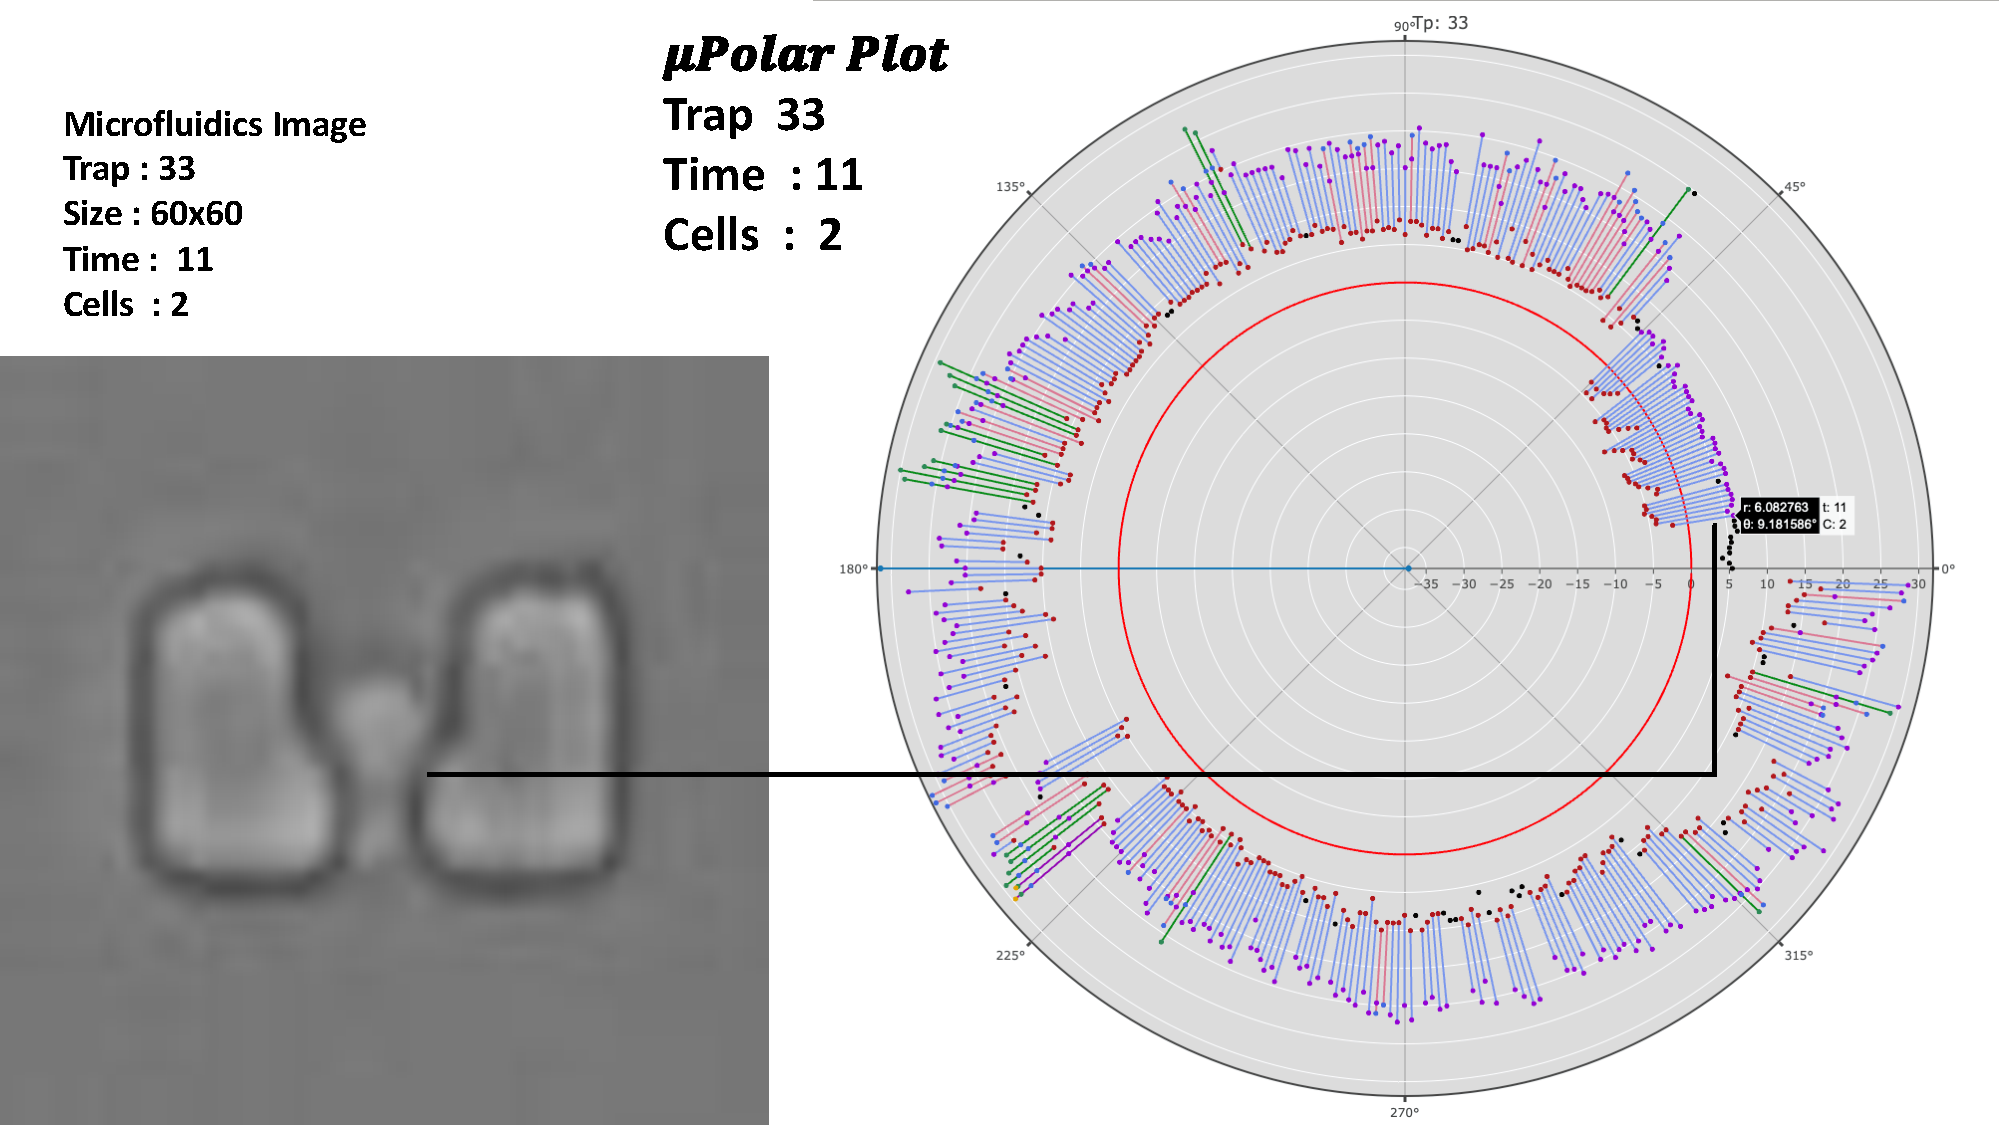
\includegraphics[width=\textwidth,height=10 cm]{Patterns/bc8tp33.pdf}
% \caption{  \textbf{$\mu$Polar visualization for Trap33 microfluidics images}.}
% \label{Fig_S2}
% \end{figure*}


\paragraph*{Fig. S4}
\label{Fig_S4}
{Oscillating patterns of cell divisions are evident in the circular plot of Trap No. 63}. 

% \begin{figure*}
% \centering
% 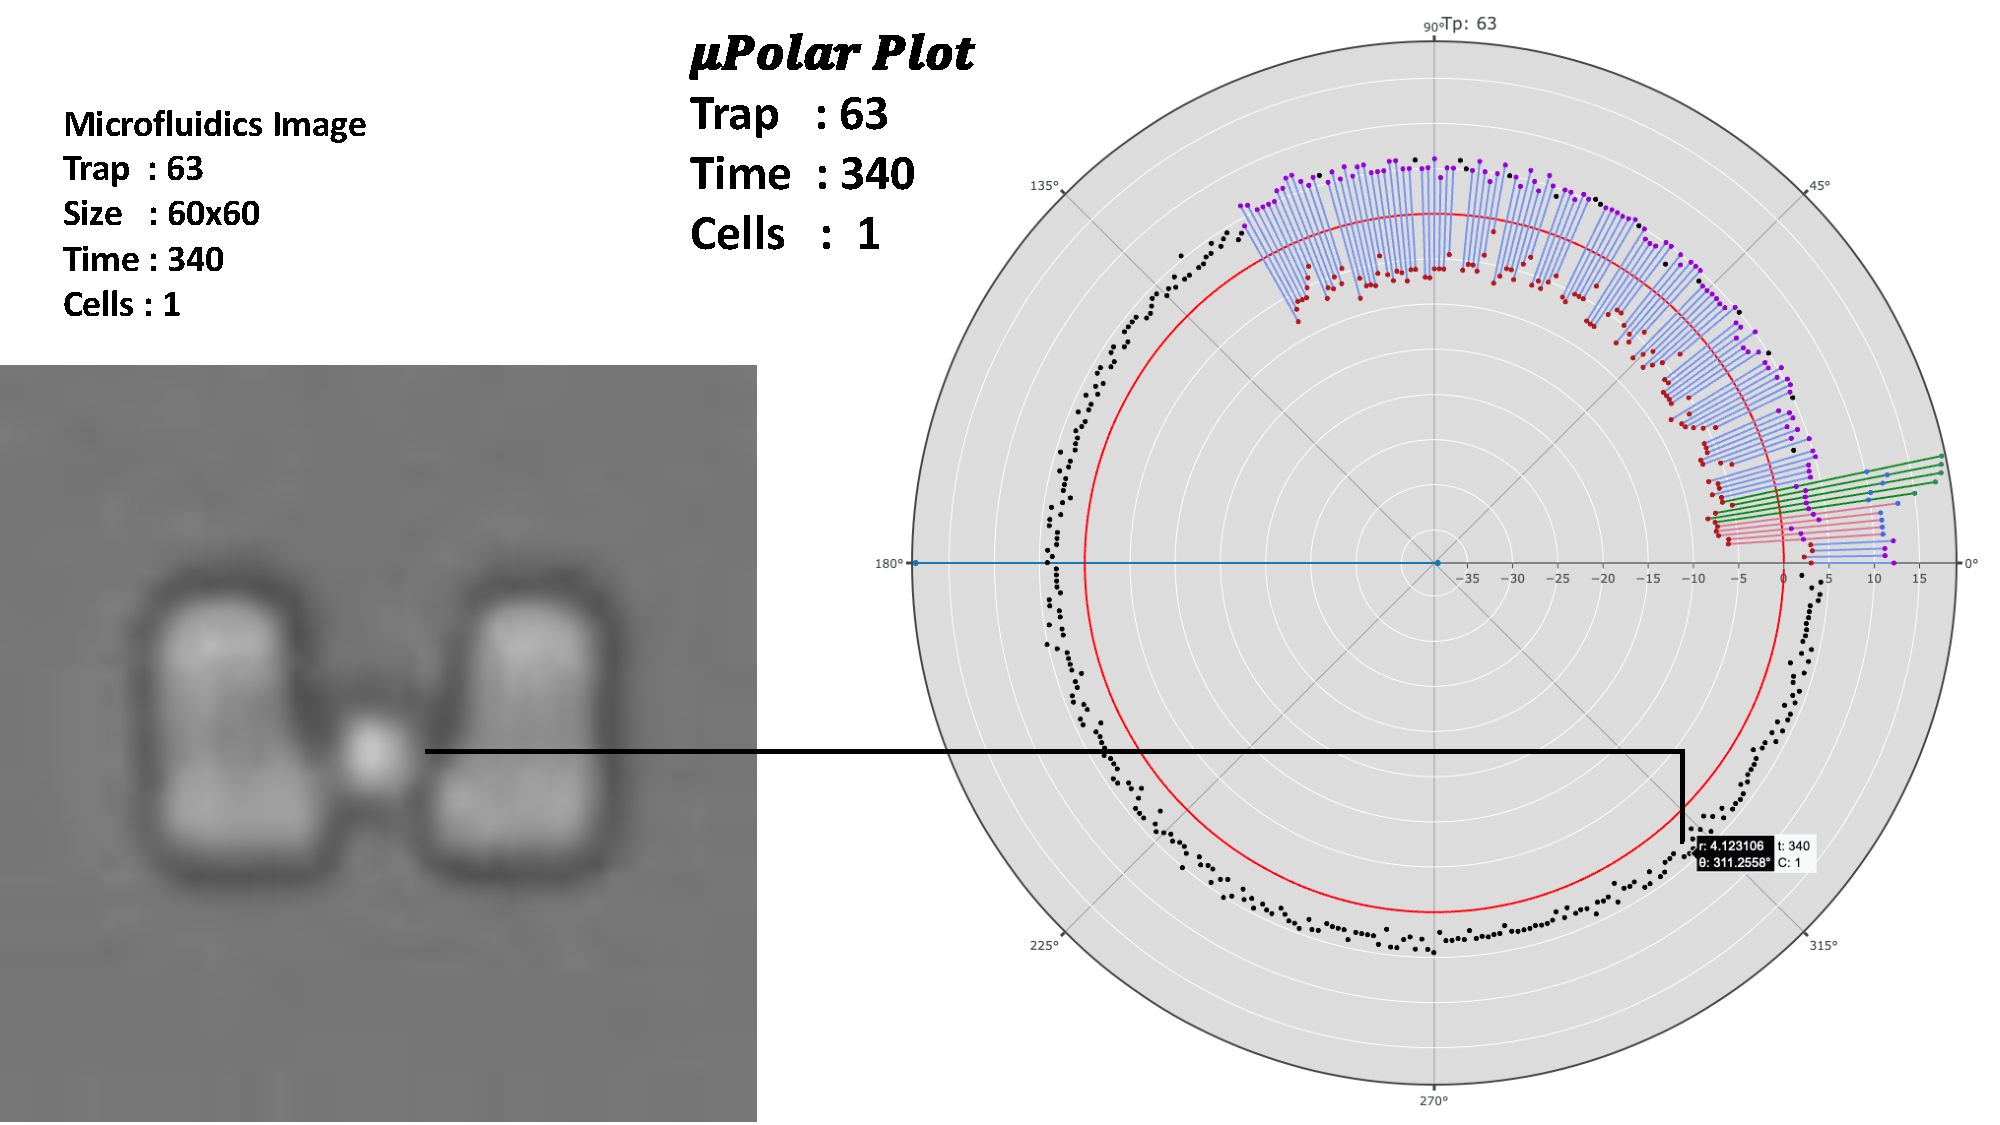
\includegraphics[width=\textwidth,height=10 cm]{Patterns/bc8tp63.pdf}
% \caption{ \textbf{$\mu$Polar visualization for Trap63 microfluidics images}.}
% \label{Fig_S4}
% \end{figure*}


\paragraph*{Fig. S5}
\label{Fig_S5}
{Illustration on how reference points can be changed to emphasize different aspects of cellular events, with Trap No. 44 as an example}. 


% \begin{figure*}
% \centering
% \includegraphics[width=\textwidth,height=10 cm]{Patterns/fluidics.pdf}
% \caption{ \textbf{HYAA microfluidics chips}. (a) Four modules (16 channels) microfluidic device. (b) A time-point sample of microfludics image shown with guidelines 10 - 70. (c) An example of time-lapse ( t1-t391) images for guidelines 10 - 20. (d) A sample of time-lapse (t1 - t391) partitioned images (60x60).}
% \label{fig:micro}
% \end{figure*}

% \paragraph*{S1 Table.}

% \label{S1_Table}
% {\bf ............} 

\section*{Acknowledgment}

The work is partially supported by NSF CAREER award \#1453078 (transferred to \#1720215), NSF award \#1761839, a  start-up fund, internal awards from the University of Tennessee at Chattanooga (Tennessee of Higher Education funds via the Center of Excellence in Applied Computational Science and Engineering), and the computing facility of the Sim center at the University of Tennessee at Chattanooga. We also acknowledge the support of NIH grants \#R01AG052507 and \#R42AG058368. We thank Dr. Weiwei Dang for sharing of yeast time-lapse image data set, Bailey S. Kirby for editorial support.

\begin{thebibliography}{00}

%%% I don't know if you care, but there are some issues in your citations. Basically: names in all caps, missing spaces, inconsistent style. -- BSK

\bibitem{r1}
Carpentera E,  Image-based chemical screening, NatureChemical Biology 3, 8 (2007), 461–465

\bibitem{r2}
Wollma R, Stuurman N,  High throughput microscopy:From raw images to discoveries, Journal of Cell Science 120, 21(2007), 3715–3722

\bibitem{r3}
Oates, A. C. et al. , Quantitative approaches in developmental biology, Nat. Rev. Genet. 10, 517–530 (2009).

\bibitem{r4}
Mavrakis M, Rikhy R, Lilly M, Lippincott-Schwartz J, Fluorescence imaging techniques for studying Drosophila embryo development, Cell Biol. 39, 4.18.1–4.18.43 (2008).

\bibitem{r5}
Amat, F. et al. ,Fast, accurate reconstruction of cell lineages from large-scale fluorescence microscopy data, Nat. Methods 11, 951–958 (2014).

\bibitem{r6}
Eliceiri KW, Berthold MR, Goldberg IG, Iba´ñez L, Manjunath BS, Martone ME, et al. Biological imaging software tools, Nat Methods. 2012; 9: 697–710. https://doi.org/10.1038/nmeth.2084 PMID: 22743775

\bibitem{r7}
McQuin C, Goodman A, Chernyshev V, Kamentsky L, Cimini BA, et al. CellProfiler 3.0: Next-generation image processing for biology, PLOS Biology 16(7), 2008, https://doi.org/10.1371/journal.pbio.2005970

\bibitem{r8}
Ghafari, M. et al. Complementary Performances of Convolutional and Capsule Neural Networks on Classifying Microfluidic Images of Dividing Yeast Cells, PLOS ONE, 2021, bioRxiv 852566; doi: https://doi.org/10.1101/852566

\bibitem{r9}
Farokhi H, Ghayesh MH (2018) Nonlinear mechanics of electrically actuated microplates, International Journal of Engineering Science 123: 197-213.

\bibitem{r10}
Jensen EC., Overview of live-cell imaging: Requirements and methods used, The Anatomical Record 296, 1 (2013),1–8


\bibitem{r11}
 Bhagat A. et al. (2010) Microfluidics for cell separation, Med Biol Eng Compu 48: 999-1014.

\bibitem{r12}
Shafiee H, Jahangir M, Inci F, Wang S, Willenbrecht RB, et al. (2013) Acute on-chip HIV detection through label-free electrical sensing of viral nano- lysate, Small 9(15): 2553-2563.

\bibitem{r13}
M. Jo, W. Liu, L. Gu, W. Dang and  L. Qin, High-throughput analysis of yeast replicative aging using a microfluidics system, Proc. Nati. Acad. Sci. USA, 2015, 112: 9364-9369.


\bibitem{r14}
H. Qin, Estimating network changes from lifespan measurements using a parsimonious gene network model of cellular aging, BMC Bioinformatics 20, 599 ,2019, doi:10.1186/s12859-019-3177-7


\bibitem{r15}
M. Ghafari,  et al. , Prototyping a family tree algorithm to estimate yeast replicative lifespan from time-lapse microfluidic images, IEEESouthEastConf. 2020, (awaiting for publication)



\bibitem{r16}
K. Steffen, B. Kennedy and M Kaeberlein, Measuring replicative life span in the budding yeast, JoVE, 2009,  28: 1-5.

\bibitem{r17}
M. Kaeberlein and B. Kennedy, Large-scale identification in yeast of conserved ageing genes, Mech Ageing Dev,2005, 126(1):17-21.

\bibitem{r18}
Buckingham, M. E,Meilhac, S. M,Tracing cells for tracking cell lineage and clonal behavior, Dev. Cell 21, 394–409 (2011).

\bibitem{r19}
R. Eilsand and C. Athale, Computational imaging in cell biology, Cell Biol.2003, 16: 477-48.

\bibitem{r20}
H. Tsai et .al, Usiigaci: Instance-aware cell tracking in stain-free phase contrast microscopy enabled by machine learnin, 2019, doi.org/10.1016/j.softx.2019.02.007.

\bibitem{r21}
S. Pang,  et al. ,A novel YOLOv3-arch model for identifying cholelithiasis and classifying gallstones on CT images, PLoS ONE, 2019, 14(6): e0217647. https://doi.org/10.1371/journal. pone.021764

\bibitem{r22}
C.  Laura, P. Hofmann, K. Drechselr  and S. Wesarg, Automatic detection of the nasal cavities and paranasal sinuses using deep neural networks, In IEEE 16th International Symposium on Biomedical Imaging,2019, pages 1154–1157. IEEE.

\bibitem{r23}
J. Martin, et al., The impact of 2D cine MR imaging parameters on automated tumor and organ localization for MR-guided real-time adaptive radiotherapy, Physics in Medicine and Biology, 2018, 63(23):235005.

\bibitem{r24}
Z. Zhao, P. Zheng, S. Xu, and X Wu, Object Detection With Deep Learning: A Review. IEEE Transactions on Neural Networks and Learning Systems, 2019, pages 1–21.


\end{thebibliography}



\end{document}
